\documentclass[12pt, oneside, a4paper]{report}

%page format
\usepackage[utf8]{inputenc}
\usepackage{titlesec}
\usepackage[left=4cm, right=3cm, top=3cm, bottom=3cm]{geometry} %set margin
\linespread{1.3} %1.5 line spacing

\titleformat{\chapter}[hang]
{\normalfont\huge\bfseries}{\chaptertitlename\ \thechapter}{0.5em}{}

%additional package
\usepackage{graphicx}
\usepackage{amsmath}
\usepackage{hyperref}
\usepackage{pdflscape}
\usepackage{caption}
\usepackage{subcaption}
\usepackage{float}
\usepackage{textcomp}
\usepackage{gensymb}
\usepackage{appendix}
\usepackage{pdfpages}
\usepackage{multicol}
\usepackage{mathtools}
\usepackage{multirow}
\usepackage{bm}
\usepackage{esvect}
\usepackage{array}
\usepackage{siunitx}
\usepackage{acro}
\usepackage{comment}
\usepackage{multirow}
\usepackage{indentfirst}
\usepackage{nomencl}
\makenomenclature
\makeindex

\usepackage[square,numbers]{natbib}
\bibliographystyle{IEEEtranN}

\renewcommand{\contentsname}{Daftar Isi}
\renewcommand{\chaptertitlename}{Bab}
\renewcommand{\figurename}{Gambar}
\renewcommand{\tablename}{Tabel}
\renewcommand*\listfigurename{Daftar Gambar}
\renewcommand*\listtablename{Daftar Tabel}
\renewcommand{\nomname}{Nomenklatur}
\renewcommand{\bibname}{Daftar Pustaka}

\begin{document}

\begin{titlepage}
    \begin{center}

        \textbf{\Large Pemodelan Termal Semi-empiris Satelit LAPAN-A3 Menggunakan Metode Machine Learning}\\
        \vspace{7em}
        \textbf{\large TUGAS SARJANA}\\
        \text{Diajukan sebagai salah satu syarat} \\
        \text{untuk memperoleh gelar Sarjana Teknik dari} \\
        \text{Institut Teknologi Bandung} \\
        
        \vspace{5em}
        Oleh\\
        Ricky Sutardi\\
        NIM : 13617051\\
       
       \vfill
       
\includegraphics[width=0.25\textwidth]{fig/logo_itb.png}
    
       \vfill
        
       \textbf{PROGRAM STUDI SARJANA TEKNIK DIRGANTARA}\\
       \textbf{FAKULTAS TEKNIK MESIN DAN DIRGANTARA}\\
       \large
       \textbf{INSTITUT TEKNOLOGI BANDUNG}\\
       \textbf{2022}\\
       
   \end{center}
\end{titlepage}

\pagenumbering{arabic}

\pagenumbering{roman}

\newpage
\addcontentsline{toc}{chapter}{Lembar Pengesahan}
\newpage

\begin{center}
       \Large
       %\textbf{Approval Page} \\
        \vspace{1.5cm}
        \large
        \textbf{Pemodelan Termal Semi-empiris Satelit LAPAN-A3 Menggunakan Metode Machine Learning}\\
        
        \vfill
        
        Oleh\\
        Ricky Sutardi\\
        NIM : 13617051\\
        (Program Studi Sarjana Teknik Dirgantara)\\
        Institut Teknologi Bandung
       
       \vfill
       
       Agustus 2022\\
        \vspace{1.0cm}
       Menyetujui\\
       \begin{multicols}{2}
       
       \footnotesize Pembimbing 1 \\
       \vspace{3.5cm}
       
        \footnotesize \textbf{\underline{Dr. Eng. Ridanto Eko Poetro ST,M.Sc.}}\\
				\footnotesize 1970004201999031002 \\
        
        \footnotesize Pembimbing 2 \\
       \vspace{3.5cm}
       
       \footnotesize  \textbf{\underline{Dr. Robertus Heru Triharjanto, M.Sc.}}\\
        \footnotesize 197110221991011001 \\
        \end{multicols}

       \footnotesize Pembimbing 3 \\
       \vspace{3.5cm}
       
       \footnotesize \textbf{\underline{Luqman Fathurrohim ST, M.T.}}\\
        \footnotesize 199401212020121003 \\
       
\end{center}


\newpage
\addcontentsline{toc}{chapter}{Abstrak}
\newpage

\begin{center}
       \Large
       \textbf{ABSTRAK} \\
        \vspace{1.5cm}
        \large
        \textbf{Pemodelan Termal Semi-empiris Satelit LAPAN-A3 Menggunakan Metode Machine Learning}\\
        
        \vspace{1.5cm}
        
        oleh\\
        Ricky Sutardi\\
        NIM : 13617051\\
        (Program Studi Sarjana Teknik Dirgantara)\\
        \vspace{1.5cm}
\end{center}

Dari pembacaan sensor suhu satelit, ditemukan bahwa LAPAN-A3, sebuah
mikrosatelit dari Indonesia, membutuhkan maneuver khusus untuk menjaga suhu
\textit{payload} utamnya, sebuah pencitra multispektral, tetap di atas 0
\degree C. Dapat disimpulkan bahwa sistem kendali termal pasif satelit tersebut
tidak cukup untuk memenuhi kebutuhan misinya. Agar permasalahan ini tidak
terjadi kembali di desain termal satelit masa depan, dibutuhkan sebuah model
termal sederhana baru yang dapat memodelkan karakteristik termal satelit
LAPAN-A3 dengan akurat.

Analisis termal satelit konvensional membutuhkan perhitungan banyak variabel
secara akurat sehingga memiliki kompleksitas yang tinggi pula. Sementara itu,
pendekatan berbasis data dalam menyelesaikan permasalahan-permasalahan termal
satelit semakin umum digunakan untuk mengurangi kompleksitas pemodelan termal
satelit. Karena itu, model termal sederhana yang dapat menghitung
parameter-parameter termal satelit yang dibutuhkan untuk memprediksi suhu
satelit dari data operasional satelit diharapkan dapat menghasilkan proses
pemodelan termal yang lebih cepat dan mudah.

Dalam karya tulis ini, model termal semi-empiris LAPAN-A3 dengan 7
\textit{node} dikembangkan dengan metode \textit{machine learning}. Model
tersebut dilatih dengan data satelit dari periode observasi 19 dan 20 Mei 2018.
Metode regresi linear menggunakan \textit{machine learning} dipilih untuk
mengurangi jumlah variabel yang harus dihitung untuk memodelkan satelit.
Evaluasi awal menunjukkan model termal secara umum dapat memprediksi perubahan
suhu \textit{node} satelit serta memiliki potensi kegunaan nyata dalam
pengembangan satelit. Meski masih dapat dikembangkan lebih lanjut, model
tersebut dapat digunakan sebagai dasar model termal satelit masa depan. 

\vspace{1.0cm}
\noindent 
Kata kunci : model termal, satelit, machine learning, regresi linear, LAPAN-A3


\newpage
\addcontentsline{toc}{chapter}{Abstract}
\begin{center}
       \Large
       \textbf{ABSTRACT} \\
        \vspace{1.5cm}
        \large
        \textbf{Semi-empirical Thermal Modelling of LAPAN-A3 Satellite Using Machine Learning Method}\\
        
        \vspace{1.5cm}
        
        by\\
        Ricky Sutardi\\
        NIM : 13617051\\
        (Bachelor's Program in Aerospace Engineering)\\
        \vspace{1.5cm}
\end{center}

From the satellite temperature sensor readings, it is found that LAPAN-A3, an
Indonesian microsatellite, requires special maneuver to keep its main payload,
a multispectral imager, above 0 \degree C. It can then be concluded that the
satellite passive thermal control system is inadequate for the satellite
mission needs. To prevent this problem in future satellite thermal design, a
new simple thermal model which can model LAPAN-A3 thermal characteristic
accurately is needed.

Conventional thermal analysis requires accurate calculations of many variable
which results in increased complexity. Meanwhile, data-driven approaches in
solving satellite thermal problem are becoming increasinly common to reduce
the complexity of thermal modelling. Thus, a simple thermal model which can
deduce the needed satellite thermal parameters to predict the satellite
temperature from existing operational satellite data hopefully can result in a
quicker and easier thermal modelling process.

In this paper, a semi-empirical 7-node thermal model of LAPAN-A3 satellite is
developed using machine learning method. The model is trained with satellite
data for the observation period of 19 and 20 May 2018. Linear regression using
machine learning is chosen to reduce the number of variables which must be
calculated to model the satellite. Initial evaluation shows that the thermal
model is generally able to predict LAPAN-A3 node temperature changes and has
potential usage in real-life satellite development. Even though the model can
still be improved upon, it may serve as a basis for future satellite thermal
model.

\vspace{1.0cm}
\noindent 
Keywords : thermal model, satellite, machine learning, linear regression, LAPAN-A3 


\chapter*{Prakata}
\addcontentsline{toc}{chapter}{Prakata}
Puji syukur penulis panjatkan kepada Tuhan Yang Maha Esa karena hanya berkat
rahmat-Nya karya tulis ini dapat diselesaikan. Karya tulis ini dibuat sebagai
syarat menyelesaikan studi pada program sarjana Teknik Dirgantara ITB. Proses
pembuatan karya tulis ini tidak lepas dari bantuan serta dukungan banyak pihak
kepada penulis. Karena itu, penulis berterima kasih kepada :

\begin{enumerate}
\item Tuhan Yang Maha Esa atas berkat kesehatan dan hikmat yang telah diberikan kepada penulis sehingga mampu menyelesaikan karya tulis ini dengan selamat.
\item Bapak Dr. Eng Ridanto Eko Poetro, Dr. Robertus Heru Triharjanto, dan Luqman Fathurrohim selaku dosen-dosen pembimbing atas semua kesabaran dalam membimbing penulis serta menjawab pertanyaan-pertanyaan yang muncul selama pengerjaan tugas akhir.
\item Keluarga yang tetap percaya penulis dapat menyelesaikan tugas akhir ini serta memberikan dukungan dan bantuan kepada penulis.
\item Teman-teman Ganesha Ipsun 17 yang menjadi pemicu semangat penulis untuk menutup kelulusan angkatan. 
\item Icarus AE17 dan seluruh massa KMPN yang menjadi rumah bagi penulis untuk tetap dapat pulang setelah lelah terbang.
\end{enumerate}

Tentu tugas akhir ini masih memiliki banyak kekurangan akibat keterbatasan
pengetahuan yang dimiliki oleh penulis. Masih banyak hal juga yang masih masih
bisa ditingkatkan dalam penelitian-penelitian selanjutnya. Oleh karena itu,
penulis berharap masukan berupa saran dan kritik dari pembaca untuk terus
memperbaiki karya tulis ini.

Terakhir, semoga karya tulis ini dapat menjadi pemrakarsa dan pemicu
pengembangan lebih lanjut dalam bidang satelit di Indonesia. Penulis juga
berharap para pembaca mendapatkan tambahan wawasan setelah membaca karya tulis
ini. Jayalah, jaya selama-lamanya!


\newpage
\addcontentsline{toc}{chapter}{Daftar Isi}
\tableofcontents

\newpage
\addcontentsline{toc}{chapter}{Daftar Gambar}
{%
\let\oldnumberline\numberline%
\renewcommand{\numberline}{\figurename~\oldnumberline}%
%\addtolength{\cftfignumwidth}{15pt}
\listoffigures%
}
%\listoffigures

\newpage
\addcontentsline{toc}{chapter}{Daftar Tabel}
{%
\let\oldnumberline\numberline%
\renewcommand{\numberline}{\tablename~\oldnumberline}%
\listoftables%
}

%list of abbreviations and symbols
%\chapter{Nomenklatur}
\newpage
\addcontentsline{toc}{chapter}{Nomenklatur}
%List of Symbols (Nomenclature)
% Latin first then Greek alphabet
% Capital (uppercase) first then lowercase

\mbox{}
\nomenclature{\(\sigma\)}{Konstanta Stefan-Boltzmann}

\printnomenclature

\printnomenclature

%Pendahuluan
\chapter{Pendahuluan}
\pagenumbering{arabic}

\section{Latar Belakang}

Pengendalian termal satelit bertujuan untuk menjaga semua komponen satelit
tetap pada rentang suhu operasional pada selama masa misi satelit. Desain
sistem kendali termal yang buruk dapat mengakibatkan kerusakan permanen pada
komponen satelit akibat panas berlebih atau kondisi non-operasional yang fatal
dalam misi akibat suhu komponen yang terlalu rendah. Semakin dekat model termal
satelit dengan karakteristik termal satelit yang sebenarnya, semakin kecil pula
kemungkinan suhu satelit mencapai nilai di luar rentang yang sudah ditentukan.
Karena itu, desain sistem kendali termal satelit yang baik membutuhkan
pemodelan termal satelit yang baik pula. Hal ini membuat proses desain sistem
kendali termal satelit menjadi salah satu tahap yang paling penting dalam
periode pengembangan satelit.

Permasalahan yang mungkin dihadapi pada proses desain sistem termal satelit
antara lain muncul karena karakteristik termal satelit ditentukan oleh banyak
parameter yang saling bergantung sama lain. Untuk memodelkan karakteristik
termal satelit secara akurat, tentunya dibutuhkan perhitungan parameter satelit
yang akurat juga. Selain itu, desain sistem kendali termal satelit harus turut
memperhitungkan batasan satelit lain seperti ruang, daya, dan berat.

Pada kasus satelit mikro dan nano, ukuran satelit yang kecil dapat berakibat
pada kapasitas termal yang kecil pula sehingga satelit mudah mengalami
perubahan suhu. Satelit mikro dan nano juga biasanya hanya bergantung pada
sistem kendali termal pasif akibat batasan ketersediaan daya. Akibatnya,
seringkali diperlukan langkah tambahan pada saat operasi untuk memastikan
satelit dapat tetap dijaga pada rentang suhu operasional. 

Permasalahan di atas terjadi pada LAPAN-A3, satelit yang memiliki misi utama
observasi Bumi serta diluncurkan pada tahun 2016. LAPAN-A3 merupakan satelit
yang dikembangkan Lembaga Penerbangan dan Antariksa Nasional (LAPAN) dengan
kerja sama dengan Institut Pertanian Bogor (IPB) setelah sebelumnya LAPAN telah
berhasil meluncurkan satelit LAPAN-A1 dan LAPAN-A2. Ketiga satelit tesebut
termasuk dalam kategori mikrosatelit serta menggunakan sistem kendali termal
pasif dengan cara distribusi panas lewat struktur dan penggunaan cat khusus
untuk memantulkan radiasi. Berbeda dengan LAPAN-A1 dan LAPAN-A2,
LAPAN-A3 membutuhkan maneuver khusus untuk menjaga suhu \textit{payload}
utamanya tetap pada rentang suhu operasional.

LAPAN-A3 memiliki \textit{payload} utama berupa pencitra multispektral yang
harus dijaga pada rentang suhu operasional 0 \degree C sampai dengan 70 \degree
C. Dari hasil observasi data telemetri, ditemukan bahwa suhu pencitra dapat
turun hingga nilai negatif dan berada pada rentang -2 \degree C dan -3 \degree
C pada periode bulan Mei sampai dengan Juni \cite{ribah2019}. Kondisi ini
berdampak buruk pada misi satelit LAPAN-A3 karena pencitra tidak dapat
dioperasikan pada suhu di bawah 0 \degree C. Akibatnya, frekuensi misi
pengambilan citra Bumi berkurang sedangkan hal tersebut merupakan misi utama
dari satelit LAPAN-A3.

Analisis lebih lanjut dari simulasi orbit satelit menemukan hubungan fenomena
penurunan suhu pencitra dengan variasi sudut antara bidang orbit satelit dan
vektor Matahari (sudut $\beta$ orbit) akibat perubahan musim seperti yang dapat dilihat pada Gambar \ref{fig:betaorbit}.

\begin{figure}[H]
\setlength\belowcaptionskip{-0.7\baselineskip}
\begin{center}
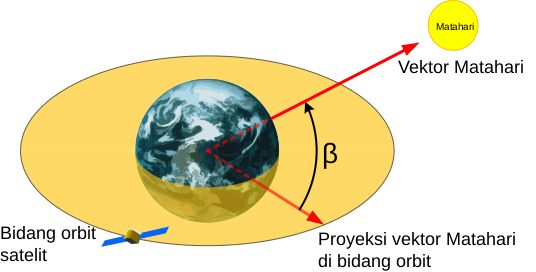
\includegraphics[width=0.7\textwidth]{fig/betaorbit.png}
\caption{Ilustrasi sudut $\beta$ orbit satelit}
\label{fig:betaorbit}
\end{center}
\end{figure}

Untuk menaikkan suhu pencitra dan melawan penurunan sudut $\beta$ tersebut,
operator LAPAN-A3 memberikan perintah maneuver \textit{stop and release} serta
\textit{stop and release with roll} sehingga sisi satelit yang memuat pencitra
menerima paparan sinar Matahari lebih banyak. Periode pemberian perintah
maneuver tidak dilakukan secara acak, tapi diatur sedemikian rupa agar satelit
dapat kembali pada sikap \textit{nadir pointing} di akhir maneuver.

Jelas dapat dilihat bahwa perlindungan termal pasif pada struktur LAPAN-A3
berupa alumunium yang telah diberi anode hitam sendiri saja tidak dapat
memenuhi persyaratan termal misi LAPAN-A3. Tanpa maneuver spesial, praktis
satelit tidak dapat menjalankan misi utamanya dengan optimal selama bulan Mei
sampai dengan Juni. Selain itu, penggunaan maneuver khusus sebagai solusi tetap
memiliki konsekuensi negatif terhadap operasi harian LAPAN-A3. 

Pertama, pencitra harus dimatikan selama durasi maneuver. Hal ini tetap
berakibat pada berkurangnya frekuensi misi pengambilan citra meski tidak
sebanyak pengurangan yang terjadi jika pencitra harus dimatikan selama bulan
Mei sampai dengan Juni. Kemudian, maneuver khusus membuat satelit terkunci
dalam sikap \textit{off-nadir pointing} selama durasi maneuver. Akibatnya, misi
yang membutuhkan sikap \textit{nadir pointing} tidak bisa dilakukan sampai
maneuver berakhir dan harus dikompensasi dengan misi lain yang tidak
membutuhkan \textit{nadir pointing} seperti pengukuran medan magnet Bumi.

Agar permasalahan yang terjadi pada satelit LAPAN-A3 saat ini tidak terulangi
pada desain satelit-satelit LAPAN di masa depan, dibutuhkan sebuah model termal
satelit yang dapat digunakan sebagai referensi dalam pengembangan
satelit-satelit LAPAN selanjutnya. Pemodelan termal satelit konvensional
dilakukan dengan menyelesaikan persamaan termal satelit yang sudah dimodelkan
menjadi beberapa titik analisis atau \textit{node} lewat perhitungan numerik
atau simulasi perangkat lunak komersial. Untuk satelit dalam kelas mikro, Das
et al. telah mengembangkan prosedur desain termal satelit sederhana menggunakan
pendekatan pertama lewat penyelesaian persamaan termal satelit \textit{node}
banyak yang disederhanakan \cite{das}. Kemudian, pendekatan kedua sudah
dilakukan oleh Boudjemai et al. yang menggunakan metode elemen hingga untuk
menganalisis karakteristik termal baterai satelit \cite{boudjemai2015}.

Karena LAPAN belum memiliki perangkat lunak yang dibutuhkan
\cite{budiantoro2019}, metode yang mungkin dipakai hanya metode perhitungan
numerik. Pendekatan ini membutuhkan perhitungan banyak parameter satelit secara
akurat bahkan untuk model satelit 1 \textit{node} sekalipun. Akibatnya, penggunaan
metode perhitungan numerik biasanya terbatas untuk model satelit 1, 2, atau 3
\textit{node} saja. 

Untuk model satelit \textit{node} banyak, pendekatan yang umum digunakan adalah
metode kedua berupa simulasi lewat perangkat lunak komersial. Sebagai contoh,
Totani et al. menjelaskan prosedur desain termal satelit kelas mikro dan nano
menggunakan metode perhitungan numerik untuk pendekatan satelit 1 dan 2
\textit{node} saja \cite{totani2014}. Pada karya tulis yang sama, prosedur
desain termal satelit dengan pendekatan model \textit{node} banyak dilakukan
dengan bantuan perangkat lunak SINDA/FLUINT. Selain itu, sampai karya tulis ini
dibuat, ketiga karya tulis yang telah disebutkan belum memberikan validasi
metode yang diajukan dengan data operasi aktual satelit.

Berdasarkan alasan yang telah dijelaskan di atas, penelitian pada karya tulis
ini bertujuan untuk menjabarkan langkah-langkah pembuatan model termal satelit
sederhana yang dapat mengurangi jumlah parameter satelit yang harus dihitung
serta dapat divalidasi dengan data telemetri satelit. Prosedur pembuatan model
termal tersebut akan diimplementasikan pada satelit LAPAN-A3. Diharapkan bahwa
model termal yang dihasilkan pada karya tulis ini dapat memprediksi suhu
satelit secara akurat sehingga satelit LAPAN di masa depan dapat memiliki
prediksi suhu komponen yang lebih akurat juga. Model termal yang lebih akurat
juga akan memungkinkan lebih banyak misi pencitraan multispektral seperti dalam
LAPAN-A4 atau \textit{payload} yang mengeluarkan panas seperti
\textit{Synthetic Apperture Radar} (SAR) pada LAPAN-A5/Chibasat.


Pada karya tulis ini, metode regresi linear berbasis \textit{machine learning} akan
digunakan untuk membuat model termal semi-empiris berbasis data telemetri
satelit aktual serta perhitungan faktor lingkungan serta orbit satelit.
Penggunaan metode \textit{machine learning} bukanlah fenomena baru dalam analisis termal
satelit. Sebagai contoh, metode \textit{machine learning} telah digunakan untuk membuat
simulasi termal satelit \textit{real-time} \cite{junior2017}, mempermudah
iterasi dalam proses desain sistem kendali termal satelit \cite{escobar2016},
serta mengoptimasi desain termal satelit \cite{xiong2020}.

Dengan demikian, diharapkan hasil akhir dari karya tulis ini adalah prosedur
pemodelan termal semi-empiris satelit LAPAN-A3 menggunakan model regresi linear
\textit{machine learning} yang dapat memprediksi suhu ke-7 \textit{node}
satelit (6 \textit{node} untuk setiap sisi satelit dan 1 \textit{node} untuk
plat tengah satelit) selama periode observasi 19 sampai dengan 20 Mei 2018.
Penggunakan metode \textit{machine learning} dilakukan untuk mengurangi jumlah
variabel yang harus dihitung untuk memodelkan karakteristik termal satelit
serta mempermudah proses perhitungan variabel yang harus dihitung. Hasil
prediksi suhu dari model termal satelit juga akan dievaluasi untuk memvalidasi
keakuratan model termal serta mengukur performa model saat ini.

\section{Rumusan Masalah}

Dari latar belakang yang telah dijelaskan sebelumnya, dapat dibuat rumusan masalah sebagai berikut :

\begin{enumerate}
\item Bagaimana pemodelan termal semi-empiris satelit LAPAN-A3 menggunakan metode \textit{machine learning} dapat dilakukan?
\item Bagaimana perbandingan perubahan suhu sisi-sisi satelit hasil prediksi model termal satelit dengan data telemetri satelit?
\item Bagaimana performa model termal satelit yang dihasilkan?
\end{enumerate}

\section{Tujuan Penelitian}

Berlandaskan rumusan masalah, penelitian pada karya tulis ini bertujuan untuk :

\begin{enumerate}
\item Melakukan penjabaran langkah-langkah untuk membuat model termal satelit \textit{node} banyak secara semi-empiris menggunakan metode \textit{machine learning}
\item Membuat model termal satelit yang dapat memprediksi perubahan suhu sisi-sisi satelit LAPAN-A3
\item Membandingkan perubahan suhu \textit{node} satelit hasil prediksi model termal dengan data telemetri satelit
\item Menganalisis performa hasil prediksi dari model termal satelit yang telah dibuat
\end{enumerate}

\section{Batasan Penelitian}

Penelitian dalam karya tulis ini dibatasi sebagai berikut :

\begin{enumerate}
\item Pemodelan termal satelit LAPAN-A3 dilakukan untuk periode observasi 19-20 Mei 2018
\item Selama periode observasi, satelit dianggap tidak mengalami perubahan massa dan karakteristik termal
\item Satelit LAPAN-A3 dianggap berbentuk balok dan dibagi menjadi 7
	\textit{node} mewakili 6 sisi satelit dan plat tengah satelit dengan aturan
		konversi sumbu menjadi nomor \textit{node} sebagai berikut : X+ = 1, X- =
		2, Y+ = 3, Y- = 4, Z+ = 5, Z- = 6, serta plat tengah = 7
\end{enumerate}

\section{Metodologi}

Gambar \ref{fig:metodologi} memuat metodologi pembuatan karya tulis ini. Secara
umum, penelitian dimulai dengan studi pustaka topik terkait pemodelan termal
satelit dan metode \textit{machine learning}. Selanjutnya, dilakukan
pengumpulan data yang dibutuhkan untuk pemodelan termal satelit. Kemudian,
dilakukan pembuatan dataset dalam format yang sesuai untuk digunakan dalam
pembuatan model \textit{machine learning}. Lalu, dataset tersebut dibagi
menjadi 2 set : set latihan untuk membantu model regresi linear \textit{machine
learning} dalam mengidentifikasi fitur dan tren perubahan suhu satelit dan set
ujian untuk mendapatkan prediksi perubahan suhu satelit dari model
\textit{machine learning}. Terakhir, hasil prediksi suhu satelit dari model
\textit{machine learning} dievaluasi untuk mengukur performa model termal saat ini.

\begin{figure}[H]
\setlength\belowcaptionskip{-0.7\baselineskip}
\begin{center}
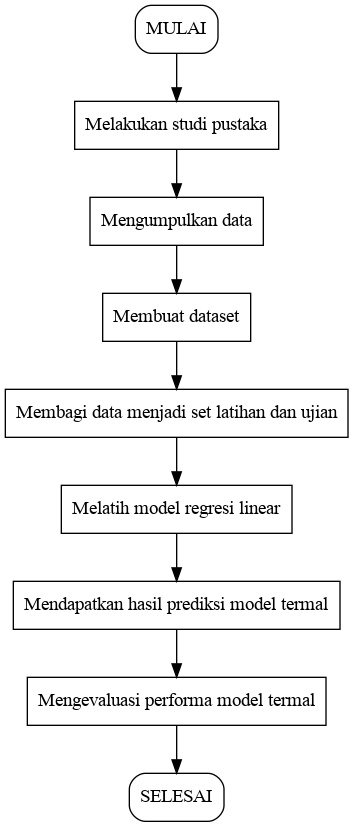
\includegraphics[width=0.4\textwidth]{fig/graph_metodologi.png}
\caption{Metodologi penelitian karya tulis}
\label{fig:metodologi}
\end{center}
\end{figure}

Proses pembuatan dataset untuk model termal satelit memiliki algoritma
tersendiri yang disajikan pada Gambar \ref{fig:algoritma}. Secara singkat,
pembuatan dataset model termal satelit terdiri dari 3 langkah utama : penyiapan
dataset dasar, perhitungan faktor-faktor panas satelit, dan penyaringan
dataset. Penjelasan lebih menyeluruh terkait proses pembuatan dataset akan
dibahas pada bab Pembuatan Model Termal Satelit LAPAN-A3.

\begin{figure}[H]
\setlength\belowcaptionskip{-0.7\baselineskip}
\begin{center}
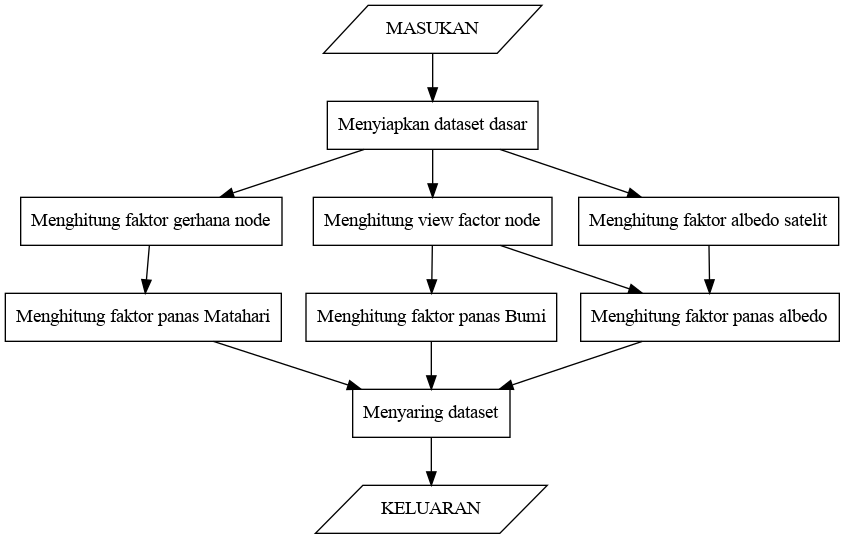
\includegraphics[width=0.75\textwidth]{fig/graph_algoritma.png}
\caption{Algoritma pembuatan dataset}
\label{fig:algoritma}
\end{center}
\end{figure}

\section{Sistematika Penulisan}

Sistematika penulisan karya tulis ini adalah sebagai berikut :

\begin{enumerate}
\item Bab 1 Pendahuluan

Bab ini membahas latar belakang, rumusan masalah, tujuan penelitian, batasan
penelitian, metodologi karya tulis, dan sistematika penulisan.

\item Bab 2 Tinjauan Pustaka

Bab ini membahas dasar teori yang digunakan dalam rangka pengerjaan karya tulis ini.

\item Bab 3 Pembuatan Model Termal Satelit LAPAN-A3

Bab ini menjabarkan langkah-langkah untuk membuat model termal semi-empiris
		satelit LAPAN-A3 dengan menggunakan metode \textit{machine learning}.

\item Bab 4 Hasil dan Analisis

Bab ini berisi hasil prediksi suhu sisi-sisi satelit LAPAN-A3 serta analisis performa model termal satelit LAPAN-A3 yang dihasilkan dari bab sebelumnya.

\item Bab 5 Kesimpulan dan Saran

Bab ini berisi kesimpulan dari penelitian yang telah dilakukan dan saran
untuk penelitian selanjutnya.
\end{enumerate}


%Dasar Teori
\chapter{Tinjauan Pustaka}

\section{Satelit LAPAN-A3}

Satelit LAPAN-A3 merupakan satelit yang diluncurkan oleh LAPAN pada 22 Juni
2016 bersama satelit CartoSat-2C milik \textit{Indian Space Research
Organization} (ISRO) dari Sriharikota, India. Satelit ini adalah satelit ketiga
yang telah diluncurkan LAPAN setelah LAPAN-A1/TUBSAT dan LAPAN-A2/ORARI serta
merupakan hasil kerja sama LAPAN dengan IPB \cite{hasbi2013}. Gambar
\ref{fig:a3overview} menunjukkan desain konfigurasi LAPAN-A3.

\begin{figure}[!ht]
\setlength\belowcaptionskip{-0.7\baselineskip}
\begin{center}
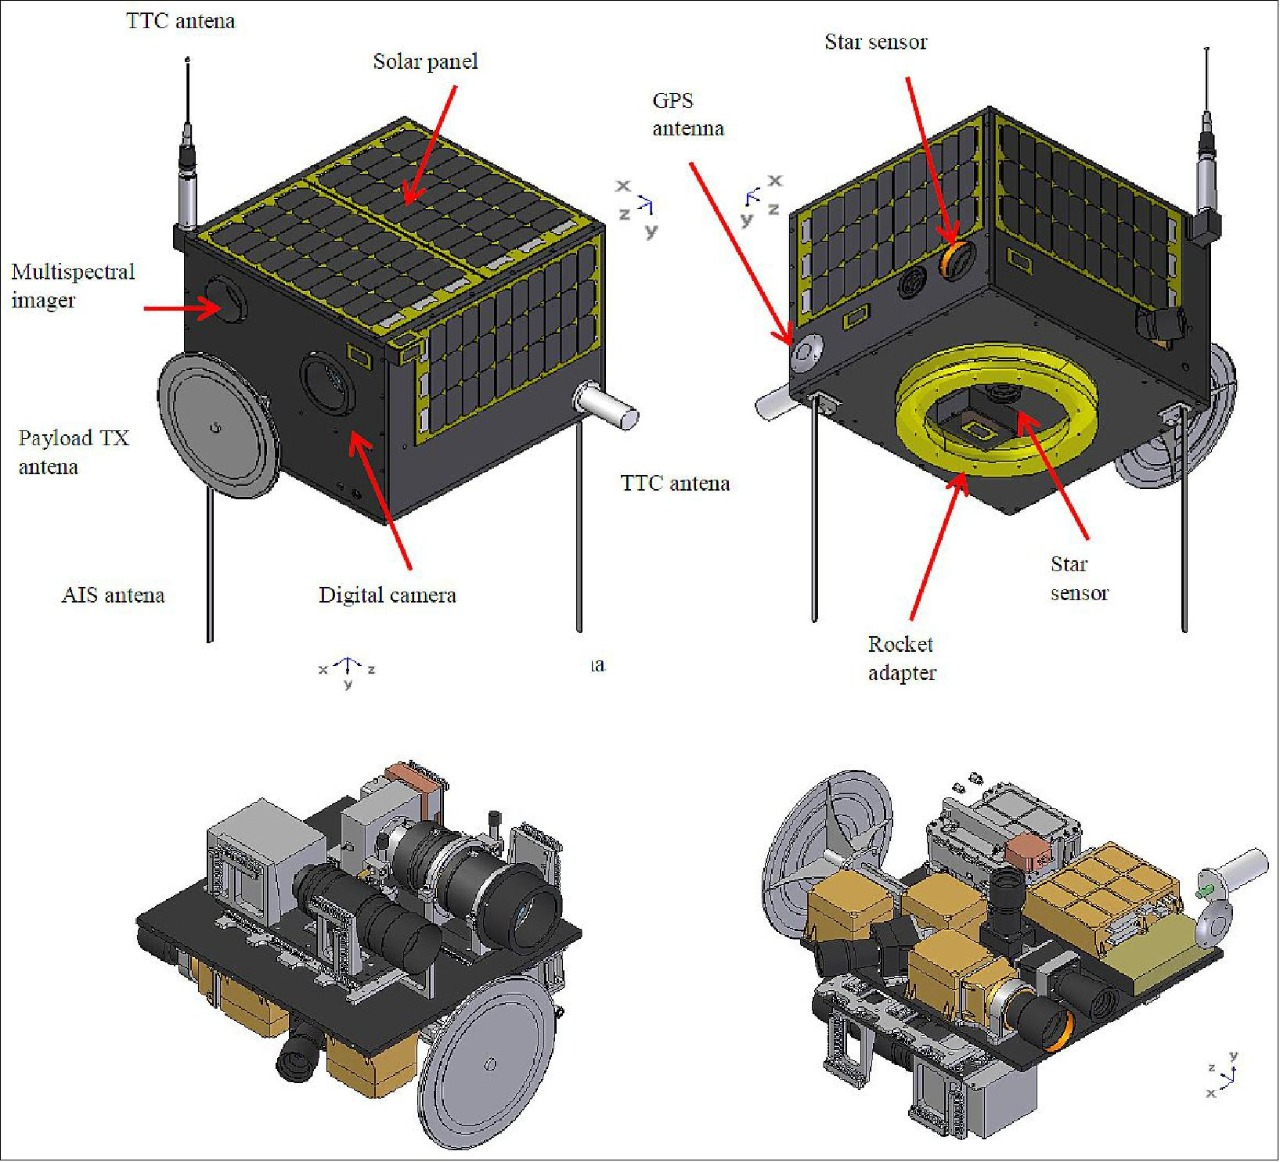
\includegraphics[width=0.7\textwidth]{fig/a3overview.jpg}
\caption{Konfigurasi LAPAN-A3}
\label{fig:a3overview}
\end{center}
\end{figure}

LAPAN-A3 memiliki misi utama untuk mendukung ketahanan pangan nasional melalui
pemantauan Bumi, khususnya di wilayah Indonesia. Untuk menyelesaikan misi
tersebut, LAPAN-A3 dilengkapi dengan instrumen pencitra multi-spekstral yang
juga dikenal sebagai \textit{Line Imager Space Application} (LISA). LISA digunakan
untuk memonitor penggunaan lahan, kondisi lingkungan, dan kesehatan tanaman panen.
Selain LISA, LAPAN-A3 juga dilengkapi \textit{Digital Space Camera} (DSC) untuk
menglibrasi LISA serta mengobservasi lebih lanjut lokasi yang diinginkan.

Selain misi pengambilan citra Bumi, LAPAN-A3 juga dilengkapi \textit{Automatic
Identification System} (AIS) untuk memonitor lalu lintas maritim. AIS dapat
mengidentifikasi kapal yang melintas di perairan Indonesia serta melacak kapal
tersebut jika terjadi pelanggaran hukum maritim. Terakhir, LAPAN-A3 juga
memiliki misi untuk mengukur medan magnet Bumi.

Orbit satelit LAPAN-A3 adalah orbit lingkaran \textit{sun-synchronous} dengan
ketinggian 515 km serta sudut inklinasi 97.5 \degree. Orbit LAPAN-A3 juga dapat
dikategorikan sebagai orbit polar dengan waktu lokal \textit{descending node}
sekitar pukul 09.30. Dalam 1 hari, LAPAN-A3 biasanya dapat melakukan kontak
dengan stasiun kendali sebanyak 2 kali (siang dan malam) selama kurang lebih 11
menit. Orbit LAPAN-A3 diatur sedemikian rupa sehingga dapat mencakup wilayah
Indonesia dan memungkinkan pengunduhan data mendekati waktu \textit{real-time}
dalam kondisi \textit{downlink}.

Kebutuhan energi satelit dipenuhi dari sinar Matahari yang ditangkap panel
surya satelit. Selain sebagai sumber energi, sinar Matahari juga digunakan
untuk memanaskan komponen satelit. Seperti yang disebutkan pada bagian Latar
Belakang sebelumnya, sistem kendali termal pasif LAPAN-A3 sendiri saja tidak
cukup untuk menjaga \textit{payload} utamanya pada suhu di atas 0 \degree C.
Dari pengumpulan data suhu LAPAN-A3 saat kondisi malam orbit serta pencitra
dimatikan, ditemukan bahwa suhu pencitra berada pada rentang nilai -2 dan -3
\degree C pada bulan Mei sampai dengan Juni. Karena itu, satelit LAPAN-A3
membutuhkan maneuver khusus agar suhu pencitra dapat dinaikkan ke atas 0
\degree C.

\section{Two-line Element}

Format data \textit{two-line element} atau TLE mendeskripsikan parameter orbit
objek ruang angkasa yang mengorbit Bumi pada suatu waktu tertentu. TLE dirilis
secara berkala ke publik oleh \textit{United States Space Command} (USSPACECOM)
yang melacak semua objek angkasa di orbit Bumi yang dapat dideteksi. Pada
praktiknya, TLE dapat digunakan untuk menghitung vektor posisi dan kecepatan
satelit yang mengorbit Bumi dengan menggunakan algoritma bernama SGP4 yang
telah ditentukan pada kode sumber TLE \cite{vallado2008}.

Algoritma SGP4 ditulis dalam bahasa pemrograman Fortran \cite{vallado2006},
tapi saat ini sudah diimplementasikan dalam banyak bahasa pemrograman lain
seperti Python. Pada karya tulis ini, TLE satelit LAPAN-A3 selama periode
observasi diambil dari situs Celestrak \cite{kelso}. TLE yang dikumpulkan
kemudian dijadikan acuan untuk propagasi orbit satelit LAPAN-A3 menggunakan
bahasa pemrograman Python lewat modul Skyfield.

\section{Persamaan Termal Satelit LAPAN-A3}

Untuk sebuah model diskrit umum satelit dengan N \textit{node} yang mengorbit
Bumi, persamaan keseimbangan termal \textit{node} $i$ yang sudah
memperhitungkan sumber masukan serta keluaran panas dan interaksi dengan
\textit{node-node} lain $j$ dapat dituliskan sebagai berikut
\cite{martinez2022}:

\begin{equation}
\label{eq:raweq}
\begin{split}
	C_{i} \frac{\Delta T_i}{\Delta t} = &\ \left(\alpha_{s,i} - \eta F_{pg,i}\right) E_s A_i \cos{\theta_{i}(t)} F_{e,i}(t) \\
	&+ \left(\alpha_{s,i} - \eta F_{pg,i}\right)\rho_{E} E_s A_i F_{i,E}(t) \cos{\beta} F_a(t) \\
	&+ \varepsilon_i A_i F_{i,E}(t) \varepsilon_E \sigma T_{i}(t)^4 \\
	&- \varepsilon_i A_i F_{i,\infty}(t) \sigma T_{i}(t)^4 \\
	&+ \mathop{\sum_{j=1}^{N}}_{j \neq i} G_{ij} \left(T_j(t) - T_i(t)\right) \\
	&+ \mathop{\sum_{j=1}^{N}}_{j \neq i} \sigma R_{ij}(T_{j}(t)^4-T_{i}(t)^4) \\
	&+ \dot{Q}_{dis,i}(t)
\end{split}
\end{equation}

dengan $C_i$ kapasitas termal rata-rata \textit{node}, $\Delta T_i$ perubahan suhu \textit{node},
$\Delta t$ selang waktu, $T_i$ suhu \textit{node}, $T_j$ suhu \textit{node-node} lain,
$\alpha_{s,i}$ absorpsi surya total \textit{node}, $\eta$ efisiensi listrik panel surya,
$F_{pg,i}$ rasio luas panel surya terhadap luas \textit{node}, $E_s$ penyinaran surya
tegak lurus terhadap arah Matahari, $A_i$ luas \textit{node}, $\theta_i$ sudut antara
garis normal permukaan \textit{node} dengan sinar Matahari, $F_{e,i}$ faktor gerhana
\textit{node}, $\rho_E$ albedo Bumi, $F_{i,E}$ \textit{view factor} \textit{node} ke Bumi, $\beta$ sudut
antara bidang orbit satelit dengan vektor Matahari, $F_a$ faktor albedo
satelit, $\varepsilon_i$ emisivitas \textit{node}, $\varepsilon_E$ emisivitas Bumi, $\sigma$
konstanta Stefan–Boltzmann, $F_{i,\infty}$ \textit{view factor} \textit{node} terhadap
lingkungan ruang angkasa, $G_{ij}$ koefisien kopling konduksi antara \textit{node} $i$
dan $j$, $R_{ij}$ koefisien kopling radiasi antara \textit{node} $i$ dan $j$, serta
$\dot{Q}_{dis,i}$ laju disipasi elektrik \textit{node}.

Pendekatan analisis termal konvensional mengharuskan perhitungan semua variabel
suku di ruas kanan Persamaan \ref{eq:raweq} untuk mendapatkan laju perubahan
suhu \textit{node} $i$. Karena pendekatan yang digunakan pada karya tulis ini adalah
regresi linear lewat metode \textit{machine learning}, Persaman \ref{eq:raweq} harus
diubah menjadi bentuk linear terlebih dahulu. Persamaan linear tersebut
nantinya akan digunakan sebagai dasar model regresi linear menggunakan metode
\textit{machine learning}.

LAPAN-A3 merupakakan satelit yang memiliki sistem kendali termal pasif serta
mengorbit Bumi secara \textit{sun-synchronous}. Dengan demikian, diasumsikan
bahwa satelit ini memiliki nilai laju disipasi elektrik $\dot{Q}_{dis,i}$ dan
\textit{view factor} \textit{node} ke lingkungan $F_{i,\infty}$ yang konstan. Satelit
LAPAN-A3 juga dilengkapi sensor sinar Matahari pada setiap sisinya
\cite{hasbi2013} sehingga sudut antara garis normal permukan \textit{node} dengan sinar
Matahari dapat dihitung berdasarkan bacaan arus sensor sinar Matahari sebagai
berikut \cite{zahran2009}:

\begin{equation}
\label{eq:current}
	\cos{\theta_i} = \frac{I_i}{I_0}
\end{equation}

dengan $I_i$ merupakan bacaan arus sensor Matahari \textit{node} dan $I_0$ arus
maksimum sensor Matahari satelit.

Selanjutnya, untuk memudahkan penulisan dan penurunan persamaan,
variabel-variabel pada 4 suku pertama Persamaan \ref{eq:raweq} yang tidak
berubah terhadap waktu selama periode observasi dapat digantikan dengan
koefisien-koefisien sesuai persamaan berikut :

\begin{equation}
\label{eq:short}
\begin{split}
	c_{S} &= \left(\alpha_{s,i} - \eta F_{pg,i}\right) E_s A_i \\
	c_{a} &= \left(\alpha_{s,i} - \eta F_{pg,i}\right)\rho_{E} E_s A_i \cos{\beta} \\
	c_{E} &= \varepsilon_i A_i \varepsilon_E \\
	c_{env} &= \varepsilon_i A_i F_{i,\infty} \sigma
\end{split}
\end{equation}

dengan $c_{S}$ merupakan koefisien suku panas akibat Matahari, $c_{a}$
koefisien suku panas akibat albedo, $c_{E}$ koefisien suku panas akibat Bumi,
dan $c_{env}$ koefisien suku disipasi ke lingkungan ruang angkasa.

Lewat substitusi nilai $\cos{\theta_i}$ dengan Persamaan \ref{eq:current} serta
koefisien-koefisien pada Persamaan \ref{eq:short} dan pembagian kedua ruas
persamaan dengan $C_i$ disertai perubahan urutan suku-suku,
Persamaan \ref{eq:raweq} dapat dijadikan persamaan linear variabel banyak
dengan ketentuan sebagai berikut :

\begin{itemize}
	\item Laju perubahan suhu \textit{node} $\frac{\Delta T_i}{\Delta t}$ sebagai variabel dependen
	\item Variabel yang berubah terhadap waktu (ditandai dengan $(t)$ pada Persamaan \ref{eq:raweq}) sebagai variabel independen
	\item Variabel yang tetap terhadap waktu sebagai gradien
	\item Konstanta suku disipasi energi $\frac{\dot{Q}_{dis,i}}{C_i}$ sebagai titik potong (\textit{intercept})
\end{itemize}

Dengan demikian, didapatkan persamaan laju perubahan suhu \textit{node} LAPAN-A3 sebagai berikut :

\begin{equation}
\label{eq:lineq}
\begin{split}
	\frac{\Delta T_i}{\Delta t} = &\ \frac{c_S}{C_i I_0} I_{i}(t) F_{e,i}(t) \\
	&+ \frac{c_a}{C_i} F_{i,E}(t) F_a(t) \\
	&+ \frac{c_E}{C_i} F_{i,E}(t) T_{i}(t)^4 \\
	&- \frac{\left( \mathop{\sum_{j=1}^{N}}_{j \neq i} \sigma R_{ij} + c_{env} \right) }{C_i} T_{i}(t)^4 \\
	&+ \mathop{\sum_{j=1}^{N}}_{j \neq i} \frac{G_{ij}}{C_i} \left(T_j(t) - T_i(t)\right) \\
	&+ \mathop{\sum_{j=1}^{N}}_{j \neq i} \frac{\sigma R_{ij}}{C_i}T_{j}(t)^4 \\
	&+ \frac{\dot{Q}_{dis,i}}{C_i}
\end{split}
\end{equation}

Persamaan \ref{eq:lineq} merupakan persamaan linear variabel banyak biasa yang
dapat diselesaikan lewat regresi linear serta akan digunakan dalam model
\textit{machine learning}. Dapat dilihat juga dari Persamaan \ref{eq:lineq} bahwa jumlah
variabel yang harus dihitung telah berkurang menjadi hanya variabel yang
berubah terhadap waktu atau hasil perkaliannya karena model regresi linear
dapat menghitung koefisien dan konstanta persamaan yang tersisa. Selain itu,
variabel seperti suhu \textit{node-node} satelit dapat langsung diketahui dari data
telemetri satelit LAPAN-A3 sehingga praktis variabel yang perlu dihitung hanya
3 faktor panas satelit. Secara singkat, Tabel \ref{table:unknown} merangkum
variabel yang masih perlu diketahui.

\begin{table}[!ht]
\begin{center}
\caption{Variabel yang masih perlu diketahui}
\label{table:unknown}
\begin{tabular}{|l|l|}
\hline
Variabel & Deskripsi \\ \hline
	$I_i F_{e,i}$        & Faktor panas akibat Matahari         \\ \hline
	$F_{i,E} F_a$        & Faktor panas akibat albedo         \\ \hline
	$F_{i,E} T_i^4$        & Faktor panas akibat Bumi         \\ \hline
	$T_i, T_j, T_i^4,$ dan $T_j^4$        & Suhu \textit{node-node} satelit         \\ \hline
\end{tabular}
\end{center}
\vspace{-5mm}
\end{table}

\section{Perhitungan Faktor Gerhana Node Satelit}

Faktor gerhana \textit{node} satelit $F_{e,i}$ diperlukan untuk menghitung faktor panas
akibat Matahari. Secara singkat, parameter ini akan bernilai 1 jika \textit{node}
menerima sinar Matahari dan sebaliknya bernilai 0 jika \textit{node} dalam fase gerhana
(tidak menerima sinar Matahari).

\section{Perhitungan View Factor Node Satelit ke Bumi}

Dalam perpindahan panas akibat radiasi, \textit{view factor} merupakan proporsi
radiasi dari suatu permukaan yang diterima oleh permukaan lain. Dengan
demikian, \textit{view factor} dari \textit{node} satelit ke Bumi merupakan
proporsi radiasi panas yang diterima permukaan Bumi dari permukaan
\textit{node} satelit. Nilai \textit{view factor} antara 2 permukaan murni
bergantung dari bentuk atau geometri kedua permukaan tersebut.

Secara umum, untuk sebuah permukaan 1 yang memancarkan radiasi ke permukaan 2 seperti yang
ditampilkan pada Gambar \ref{fig:viewfactor}, \textit{view factor} dari
permukaan 1 ke 2 $F_{1,2}$ dapat ditentukan lewat persamaan berikut
\cite{muneer2020}:

\begin{equation}
\label{eq:viewfactor}
	F_{1,2} = \frac{1}{A_1} \int_{A_1} \int_{A_2} \frac{\cos{\Phi_1} \cos{\Phi_2}}{\pi R_{12}} dA_2 dA_1
\end{equation}

dengan $A_1$ merupakan luas permukaan 1, $A_2$ luas permukaan 2, $dA_1$ elemen
diferensial permukaan 1, $dA_2$ elemen diferensial permukaan 2, $R_{12}$ jarak
antara $dA_1$ dan $dA_2$, dan $\Phi_1$ serta $\Phi_2$ sudut antara vektor
normal masing-masing elemen diferensial permukaan dengan garis $R$.  

\begin{figure}[!ht]
\setlength\belowcaptionskip{-0.7\baselineskip}
\begin{center}
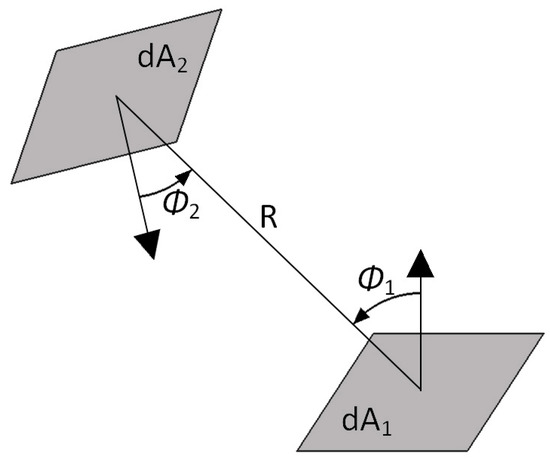
\includegraphics[width=0.5\textwidth]{fig/viewfactor.jpg}
	\caption{Ilustrasi geometri perhitungan \textit{view factor}}
\label{fig:viewfactor}
\end{center}
\end{figure}

Solusi analitik Persamaan \ref{eq:viewfactor} hanya tersedia
untuk kasus bentuk permukaan sederhana seperti plat, bola, dan tabung.
Untuk bentuk permukaan yang lebih kompleks, Persamaan
\ref{eq:viewfactor} harus diselesaikan secara numerik semisal
menggunakan metode Monte-Carlo, perangkat lunak komersial yang memang
dirancang untuk menghitung \textit{view factor} geometri kompleks,
atau metode numerik lainnya.

Dari bagian Batasan Penelitian, satelit LAPAN-A3 diasumsikan berbentuk
balok. Dengan demikian, \textit{node} yang mewakili sisi-sisi
satelit dapat dianggap berbentuk plat persegi panjang. Selanjutnya, ukuran
satelit jauh lebih kecil dari Bumi sehingga sisi satelit dapat didekati dengan
elemen diferensial plat persegi panjang terhadap Bumi. Dengan begitu, nilai
\textit{view factor} \textit{node} satelit ke Bumi dapat didekati
dengan perhitungan analitik bentuk dasar plat persegi panjang
(\textit{node}) ke bola (Bumi). 

Semisal, akan dicari nilai \textit{view factor} dari permukaan plat persegi
panjang ke permukaan bola dengan jari-jari $r$ seperti yang ditampilkan pada
Gambar \ref{fig:platball}. Variabel $\gamma$ merupakan sudut antara vektor
normal permukaan plat $\hat{n}$ dengan garis jarak antara kedua permukaan $H$.

\begin{figure}[!ht]
\setlength\belowcaptionskip{-0.7\baselineskip}
\begin{center}
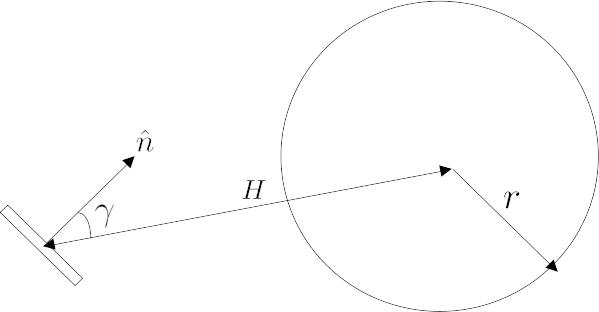
\includegraphics[width=0.5\textwidth]{fig/platball.png}
	\caption{Ilustrasi \textit{view factor} dari plat ke bola}
\label{fig:platball}
\end{center}
\end{figure}

Untuk mempermudah perhitungan \textit{view factor}, akan didefinisikan 3 variabel sebagai berikut :

\begin{equation}
\begin{split}
\label{eq:hxy}
	h &\equiv \frac{H}{r} \\
	x &\equiv \sqrt{h^2 - 1} \\
	y &\equiv -x \cot{\gamma}
\end{split}
\end{equation}

Nilai \textit{view factor} dari permukaan plat persegi panjang 1 ke permukaan
bola 2 kemudian dapat dihitung berdasarkan persamaan berikut \cite{martinez2022a}:

\begin{equation}
	F_{1,2} = 
\begin{cases} 
	\frac{\cos{\gamma}}{h^2} & ,\;|\gamma| \leq \cos^{-1}\left(\frac{1}{h}\right) \\
	\frac{1}{\pi h^2} \left( \cos{\gamma}\cos^{-1}y - x\sin{\gamma}\sqrt{1-y^2} \right) + \frac{1}{\pi}\tan^{-1}\left( \frac{\sin{\gamma}\sqrt{1-y^2}}{x} \right) & ,\;|\gamma| > \cos^{-1}\left(\frac{1}{h}\right) \\
\end{cases}
\label{eq:vf}
\end{equation}

\section{Perhitungan Faktor Albedo}

Masukan panas dari albedo pada satelit bersumber dari radiasi sinar Matahari
yang dipantulkan benda langit seperti planet, bulan, atau wahana antariksa
lain. Pada LAPAN-A3, albedo yang diterima satelit berasal dari sinar Matahari
yang dipantulkan oleh Bumi. Karena itu, faktor albedo LAPAN-A3 mewakili
proporsi radiasi pantulan yang diterima satelit dari Bumi. Faktor albedo
satelit bernilai 0 saat satelit memasuki fase gerhana dan bernilai 1 saat
satelit berada pada titik \textit{subsolar}, titik di orbit satelit yang
memiliki jarak paling dekat dengan Matahari. 

Secara umum, faktor albedo satelit dapat dituliskan sebagai berikut :

\begin{equation}
\label{eq:albedofactor}
F_a = \left( \frac{1 + \cos{\phi}}{2} \right)^2 \left[ 1 - \left( \frac{\phi}{\phi_{es}} \right)^2 \right] F_e
\end{equation}

dengan $\phi$ merupakan posisi sudut satelit, $\phi_{es}$ posisi sudut satelit
saat memasuki fase gerhana, dan $F_e$ faktor gerhana satelit. Kedua posisi
sudut dihitung dari titik \textit{subsolar}. Faktor gerhana satelit sendiri
bernilai 0 jika satelit dalam fase gerhana dan sebaliknya bernilai 1 jika
satelit tidak dalam fase gerhana.

\section{Machine Learning}

Bidang \textit{machine learning} secara umum mempelajari metode dan algoritma
komputer yang dapat menggunakan data untuk meningkatkan performa dalam
mengerjakan serangkaian tugas secara otomatis \cite{mitchell1997}. Sebuah model
\textit{machine learning} mampu mempelajari sendiri karakteristik permasalahan
yang perlu diselesaikan dari kumpulan data yang diberikan tanpa intervensi
operator manusia. Karena itu, metode \textit{machine learning} sudah umum
digunakan dalam penyelesaian berbagai permasalahan dalam bidang-bidang lain.
Sebagai contoh, pengelompokan wajah manusia, pembuatan rekomendasi produk, dan
analisis finansial modern lazim menggunakan metode \textit{machine learning}

\subsection{Aplikasi Machine Learning Dalam Pemodelan Termal Satelit}

Aplikasi metode \textit{machine learning} dalam analisis termal secara umum
dapat dibagi menjadi 2 : inferensi dan prediksi. Inferensi merupakan proses
pembuatan model matematis yang menggambarkan hubungan variabel-variabel dalam
cara kerja suatu sistem sedangkan prediksi adalah proses pembuatan prakiraan
hasil masa depan atau variabel yang belum diobservasi berdasarkan data
observasi yang sudah ada. Dalam konteks pemodelan termal satelit, inferensi
dapat digunakan untuk menghitung kontribusi tiap suku dalam persamaan termal
satelit sehingga dampak masing-masing suku secara individual dapat diketahui.
Prediksi sendiri dapat digunakan untuk menentukan besaran parameter termal yang
sebelumnya tidak diketahui berdasarkan parameter yang sudah diketahui.

Dalam karya tulis ini, prediksi menggunakan metode \textit{machine learning}
akan digunakan untuk menyelesaikan persamaan laju perubahan suhu \textit{node}
satelit seperti yang dituliskan pada Persamaan \ref{eq:lineq}. Secara spesifik,
metode \textit{machine learning} yang digunakan adalah pemodelan regresi linear
menggunakan bahasa pemrograman Python yang dilatih menggunakan data TLE beserta
data telemetri satelit LAPAN-A3 untuk periode observasi 19 dan 20 Mei 2018.
Mirip dengan regresi linear dalam statistik, model regresi linear
\textit{machine learning} akan menghitung koefisien suku-suku pada Persamaan
\ref{eq:lineq} yang belum diketahui berdasarkan data masukan model
\textit{machine learning}. Hasil perhitungan koefisien suku-suku termal
tersebut kemudian akan digunakan untuk memprediksi laju perubahan suhu
\textit{node} dataset ujian model. Lewat prediksi laju perubahan suhu
\textit{node}, perubahan suhu \textit{node} dan suhu \textit{node} pada selang
waktu pengamatan berikutnya dapat diprediksi juga.

\subsection{Evaluasi Performa Model Machine Learning}

Performa model termal satelit dapat diukur dari kemampuan model untuk
memprediksi tren perubahan suhu satelit serta keakuratan model dalam
memprediksi nilai perubahan suhu satelit. Untuk mengevaluasi performa prediksi
model regresi linear, dapat digunakan skor koefisien determinasi ($R^2$)
\cite{gupta2021} dan nilai \textit{root mean squared error} (RMSE)
\cite{zheng}. Perhitungan skor $R^2$ dan nilai RMSE sesuai konteks model
\textit{machine learning} sudah tersedia pada modul \textit{machine learning}
dalam bahasa pemrograman Python yang dipakai dalam karya tulis ini sehingga
sub-bagian ini hanya akan mendeskripsikan kedua parameter tersebut.

Skor koefisien determinasi atau $R^2$ mengukur seberapa baik model regresi
memprediksi tren data observasi. Parameter ini bernilai maksimum 1 dan semakin
tinggi skor $R^2$, semakin dekat tren hasil prediksi model dengan tren data
observasi. Skor ini juga mengukur proporsi varians dalam data observasi yang
dapat dijelaskan oleh hasil prediksi model. Sebagai contoh, jika hasil prediksi
model regresi memiliki skor $R^2$ senilai 0.9, 90\% varians dalam data
observasi dapat dijelaskan oleh hasil prediksi model.

Nilai \textit{root mean squared error} atau RMSE mengukur seberapa besar
perbedaan antara hasil prediksi model dengan data observasi. RMSE selalu
bernilai positif dan semakin rendah nilai RMSE, semakin dekat pula prediksi
model regresi dengan data observasi. Parameter ini bergantung pada skala data
serta dataset yang digunakan oleh model. Karena itu, parameter ini dapat
dijadikan pembanding akurasi antara model-model yang memiliki dataset masukan
yang sama.

\section{Perangkat Lunak}

\subsection{Python}

Python adalah bahasa pemrograman umum yang diciptakan oleh Guido van
Rossum. Python umum digunakan untuk menyelesaikan permasalahan sains
data. Bahasa ini dipilih untuk melakukan perhitungan dan
pemodelan dalam karya tulis ini karena memiliki modul pemrograman yang
cukup lengkap, tidak terikat biaya lisensi, dan kode sumber-nya dapat
diakses secara publik. Versi bahasa Python yang digunakan pada karya
tulis ini adalah 3.10.

\subsection{Pandas}

Pandas adalah modul pemrogaman untuk bahasa Python yang diciptakan oleh Wes
McKinney. Modul ini biasa digunakan untuk mengolah dan menganalisis objek data
seperti baris dan kolom tabel \cite{reback2022}. Pada karya tulis ini, modul Pandas
digunakan untuk mengolah sumber data mentah berupa data telemetri satelit LAPAN
A3 agar dapat diproses lebih lanjut pada tahap pembuatan model termal satelit.

\subsection{Numpy}

Numpy adalah sebuah modul Python yang diciptakan oleh Travis Oliphant. Modul
ini digunakan untuk melakukan operasi pada matriks multi-dimensional secara
cepat dan efisien \cite{harris2020}. Karya tulis ini menggunakan Numpy untuk
menghitung dan menyimpan variabel-variabel yang dibutuhkan model termal satelit
seperti matriks sudut Euler satelit, matriks posisi satelit, dan lain-lain. 

\subsection{Matplotlib}

Matplotlib adalah modul Python untuk membuat plot dan grafik 2D \cite{hunter2007}.
Modul ini diciptakan oleh John Hunter dan umum digunakan pada proyek sains data
sebagai sarana visualisasi data. Karya tulis ini menggunakan modul Matplotlib
untuk menggambarkan hasil pemodelan termal satelit.

\subsection{Scikit-learn}

Scikit-learn merupakan modul pengolahan data, pembuatan model, validasi, dan
pengukuran performa model \textit{machine learning} dalam bahasa Python \cite{pedregosa2011}.
Modul ini pertama kali dikembangkan oleh David Cournapeau pada 2007 dan
mencakup algoritma-algoritma \textit{machine learning} untuk skala menengah.
Scikit-learn digunakan untuk pembuatan model \textit{machine learning} pada karya tulis
ini.

\subsection{Skyfield}

Skyfield adalah sebuah modul astronomi untuk perhitungan posisi bintang,
planet, dan satelit yang mengorbit di sekitar Bumi [@rhodes2019]. Modul ini
ditulis oleh Brandon Rhodes dan menggunakan implementasi algoritma SGP4 dalam
bahasa Python \cite{rodriguez} untuk memprediksi dinamika orbit satelit mengacu
format TLE. Karya tulis ini menggunakan Skyfield untuk
mensimulasikan orbit LAPAN-A3 selama periode observasi.

\subsection{Scipy}

Scipy adalah sebuah modul perhitungan saintifik dalam bahasa Python yang
dikembangkan pertama kali oleh Travis Oliphant, Pearu Peterson, dan Eric Jones
\cite{virtanen2020}. Modul ini memuat formula perhitungan aljabar, persamaan
diferensial, statistik, dan formula-formula umum lain. Pada karya tulis ini,
Scipy digunakan untuk menghitung skor standar data suhu \textit{node} satelit
untuk mendeteksi data \textit{outlier}.


%Pemodelan Termal
\chapter{Pembuatan Model Termal Satelit LAPAN-A3}

Bab ini akan membahas langkah-langkah untuk membuat model termal semi-empiris
satelit LAPAN-A3 menggunakan metode \textit{machine learning}. Diagram alir
proses pembuatan model termal tersebut dapat dilihat kembali pada Gambar
\ref{fig:metodologi} yang memuat metodologi penelitan pada karya tulis ini
secara umum. Kemudian, karena persamaan-persamaan terkait perhitungan variabel
model termal sudah dibahas secara menyeluruh pada bab Tinjauan Pustaka, bab ini
hanya akan membahas bagaimana variabel pada persamaan-persamaan tersebut dapat
dihitung dari data yang sudah dikumpulkan. Penjabaran fungsi dan algoritma
dalam pembuatan model termal lebih mendalam dapat dilihat di kode sumber
pemrograman karya tulis ini yang tersedia di repositori \textit{Github}
https://github.com/sutricky/a3thermalmodel.

\section{Pengumpulan Data}

Data untuk penelitian di karya tulis ini dapat dibagi menjadi 2 jenis : data
telemetri satelit LAPAN-A3 serta data \textit{two-line elements} (TLE). Data
telemetri satelit LAPAN-A3 diperoleh dari data operasional internal LAPAN,
sedangkan data TLE LAPAN-A3 diambil dari situs Celestrak \cite{kelso}. Kedua
jenis data dikumpulkan untuk periode observasi 19 sampai dengan 20 Mei 2018.
Contoh data telemetri satelit LAPAN-A3 dapat dilihat pada Gambar
\ref{fig:telea3} dan contoh data TLE LAPAN-A3 dapat dilihat pada Gambar
\ref{fig:tlea3}.

\begin{figure}[H]
\setlength\belowcaptionskip{-0.7\baselineskip}
\begin{center}
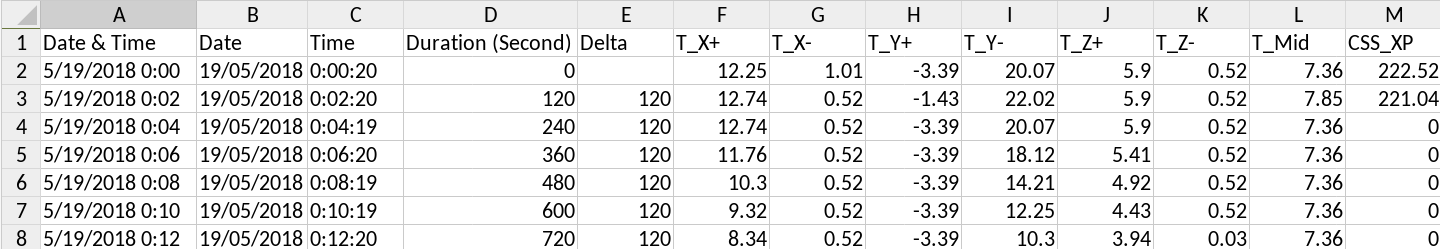
\includegraphics[width=0.8\textwidth]{fig/telea3.png}
\caption{Contoh data telemetri LAPAN-A3}
\label{fig:telea3}
\end{center}
\end{figure}

\begin{figure}[H]
\setlength\belowcaptionskip{-0.7\baselineskip}
\begin{center}
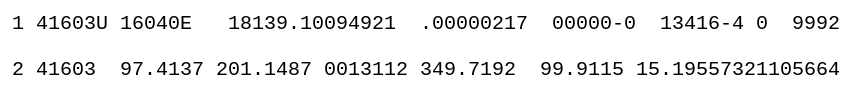
\includegraphics[width=0.7\textwidth]{fig/tlea3.png}
\caption{Contoh data TLE LAPAN-A3}
\label{fig:tlea3}
\end{center}
\end{figure}

Data telemetri satelit LAPAN-A3 yang dibutuhkan mencakup pembacaan sensor suhu
dan sinar Matahari \textit{node-node} satelit serta sikap satelit selama
periode observasi. Sesuai dengan model satelit LAPAN-A3 yang digunakan, data
yang disediakan oleh LAPAN juga sudah berupa bacaan sensor dari 6 sisi satelit
dan plat tengah satelit.

Selanjutnya, nilai TLE satelit diasumsikan tidak berubah selama 1 periode
observasi. Karena itu, \textit{epoch} atau waktu acuan yang digunakan untuk
perhitungan orbit satelit selama 1 hari pada bagian berikutnya adalah data TLE
pertama yang tersedia pada periode observasi sesuai zona waktu UTC. Asumsi ini
didasari oleh algoritma SGP-4 yang digunakan untuk mempropagasi orbit satelit
LAPAN-A3 memiliki akurasi yang cukup untuk memprediksi orbit satelit dalam
rentang waktu 15 hari dari waktu acuan \cite{kelsoa}. Secara spesifik untuk
LAPAN-A3, selisih kesalahan rata-rata perhitungan posisi LAPAN-A3 yang
menggunakan data TLE terbaru dan data TLE 1 hari sebelumnya bernilai 0.364 km
\cite{nugroho2018}. 

\section{Pembuatan Dataset}

Sebagai gambaran umum, diagram alir yang ditunjukkan Gambar \ref{fig:algoritma}
pada bagian Metodologi memperlihatkan \textit{pipeline} data dalam pembuatan
dataset untuk model \textit{machine learning}. Pembuatan dataset dilakukan
dengan mempersiapkan dataset dasar, menghitung faktor termal satelit, dan
menyaring dataset.

\subsection{Persiapan Dataset Dasar}

Data mentah yang sudah dikumpulkan di tahap sebelumnya diproses terlebih dahulu
lewat kode Python sehingga memiliki bentuk dan satuan yang sesuai untuk
diproses lebih lanjut di tahap berikutnya. Proses ini dilakukan hanya pada data
mentah telemetri satelit LAPAN-A3 karena data TLE sudah dalam format yang dapat
digunakan oleh modul Skyfield. Secara singkat, data bacaan sensor suhu
\textit{node} satelit diubah menjadi satuan K, bacaan arus pada sensor Matahari
menjadi satuan A, dan sikap satelit menjadi satuan rad. Selain itu, data
perubahan suhu \textit{node} satelit antar selang waktu observasi juga turut
dihitung. Kemudian, data waktu pembacaan sensor-sensor satelit dipisah menjadi
format tahun, bulan, tanggal, jam, menit, dan detik untuk memudahkan propagasi
orbit di bagian berikutnya. Gambar \ref{fig:basedataset} menunjukkan
contoh dataset dasar yang dihasilkan dari kode Python.

\begin{figure}[H]
\setlength\belowcaptionskip{-0.7\baselineskip}
\begin{center}
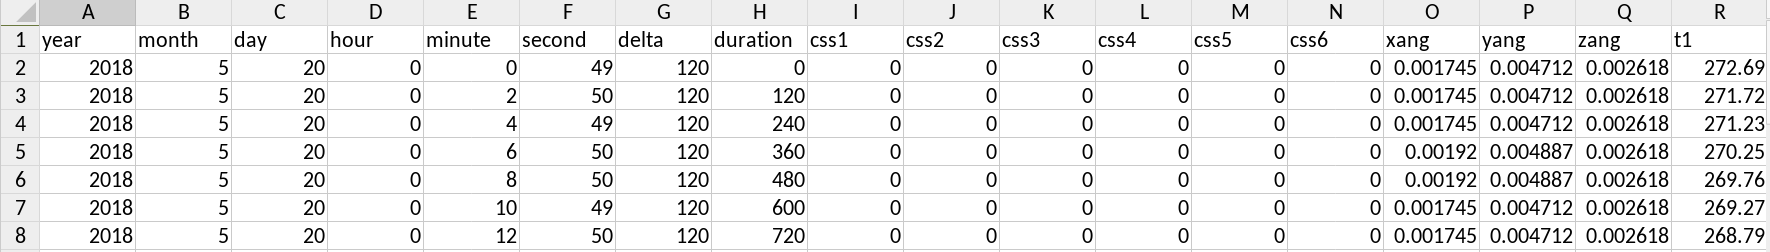
\includegraphics[width=0.8\textwidth]{fig/basedataset.png}
\caption{Contoh dataset dasar keluaran kode Python}
\label{fig:basedataset}
\end{center}
\end{figure}

\subsection{Perhitungan Faktor Termal Satelit}

Sesuai diagram alir \textit{pipeline} yang ditunjukkan Gambar
\ref{fig:algoritma} dan tabel variabel yang masih belum diketahui pada Tabel
\ref{table:unknown}, perhitungan faktor termal satelit terbagi mencakup 3 jenis
variabel : faktor panas akibat Matahari, Bumi, dan albedo. Ketiga jenis
variabel tersebut dihitung juga menggunakan kode Python. 

Pertama, faktor panas akibat Matahari merupakan hasil perkalian bacaan arus
sensor Matahari \textit{node} dan faktor gerhana \textit{node} satelit. Sejalan
dengan definisi faktor gerhana node yang dijelaskan pada bab Tinjauan Pustaka,
nilai variabel tersebut dapat ditentukan dari pembacaan arus sensor sinar
Matahari \textit{node} terkait; bacaan arus lebih besar dari 0 A berarti
\textit{node} menerima sinar Matahari sehingga memiliki nilai faktor gerhana
sebesar 1. Sebaliknya, jika bacaan arus sensor \textit{node} bernilai 0,
\textit{node} tidak menerima sinar Matahari sehingga memiliki nilai faktor
gerhana 0.

Perhitungan faktor gerhana \textit{node} dari data arus sensor Matahari
\textit{node} harus memperhatikan toleransi kesalahan bacaan sensor yang
mungkin terjadi. Sebagai contoh, sensor Matahari pada satelit LAPAN-A3 yang
digunakan dalam karya tulis ini menunjukkan pembacaan lebih besar dari 0 A pada
beberapa selang waktu pengamatan meskipun seharusnya satelit berada pada fase
gerhana merujuk pada nilai bacaan arus sensor \textit{node} sebelum dan
sesudahnya. Bacaan arus sensor Matahari \textit{node} tersebut dapat dianggap
kesalahan pengukuran karena terjadi konsisten pada setiap sensor dengan besar
yang sama dan hanya terjadi pada beberapa selang waktu tertentu saat satelit
jelas dalam fase gerhana. Gambar \ref{fig:solarfactor} menunjukkan contoh hasil perhitungan faktor panas akibat Matahari. 

\begin{figure}[H]
\setlength\belowcaptionskip{-0.7\baselineskip}
\begin{center}
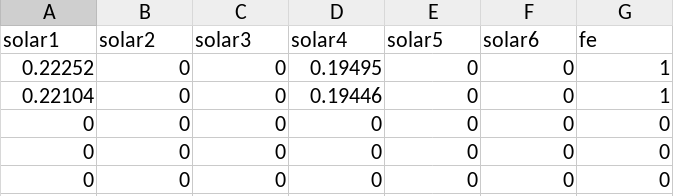
\includegraphics[width=0.6\textwidth]{fig/solarfactor.png}
\caption{Contoh hasil perhitungan faktor panas akibat Matahari}
\label{fig:solarfactor}
\end{center}
\end{figure}

Selanjutnya, faktor panas akibat Bumi dan albedo sama-sama bergantung pada
perhitungan \textit{view factor} \textit{node} satelit ke Bumi. Sesuai dengan
Persamaan \ref{eq:vf}, \textit{view factor} dari \textit{node} satelit ke Bumi
didekati dengan \textit{view factor} dari plat persegi panjang ke bola. Persamaan \ref{eq:vf} membutuhkan jari-jari bola $r$, jarak antara plat dengan bola $R$, dan sudut antara garis normal permukaan plat dengan garis jarak antara plat dan bola $\gamma$. 

Jari-jari bola $r$ dapat didekati dengan nilai rata-rata jari-jari Bumi sebesar
6371 km \cite{moritz}. Lalu, karena ukuran satelit jauh lebih kecil dari Bumi,
jarak plat ke bola $H$ dapat didekati dengan jarak antara satelit dan Bumi yang
dapat dihitung dengan mempropagasi orbit satelit berdasarkan data TLE
menggunakan modul Skyfield. Propagasi orbit lewat modul Skyfield juga
memungkinkan perhitungan vektor posisi satelit seiring perubahan waktu. Dengan
demikian, sudut antara garis normal permukaan plat dengan bola $\gamma$ dapat
didekati dengan sudut antara vektor normal permukaan \textit{node} dengan
vektor posisi satelit terhadap Bumi. 

Perhitungan sudut $\gamma$ perlu memperhatikan tata acuan koordinat yang
digunakan pada kedua vektor. Pada perhitungan \textit{view factor node} di
karya tulis ini, sistem koordinat yang digunakan adalah sistem koordinat bawaan
modul Skyfield yaitu \textit{Geocentric Celestial Reference System} (GCRS).
Karena itu, vektor normal permukaan \textit{node} harus dikonversi terlebih
dahulu dengan bantuan matriks rotasi sudut Euler dengan urutan Z-Y-X. Gambar
\ref{fig:vffig} menunjukkan contoh hasil perhitungan \textit{view factor node}
satelit ke Bumi dan Gambar \ref{fig:earthfactor} menunjukkan contoh hasil perhitungan faktor panas akibat Bumi.

\begin{figure}[H]
\setlength\belowcaptionskip{-0.7\baselineskip}
\begin{center}
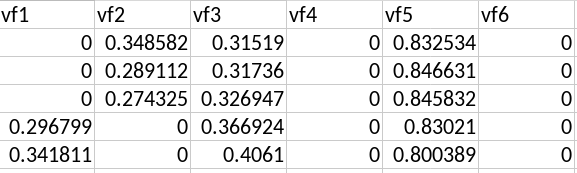
\includegraphics[width=0.6\textwidth]{fig/vffig.png}
\caption{Contoh hasil perhitungan \textit{view factor node} satelit ke Bumi}
\label{fig:vffig}
\end{center}
\end{figure}

\begin{figure}[H]
\setlength\belowcaptionskip{-0.7\baselineskip}
\begin{center}
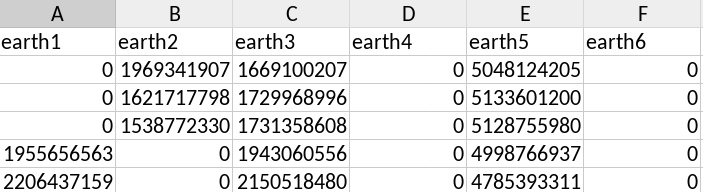
\includegraphics[width=0.6\textwidth]{fig/earthfactor.png}
\caption{Contoh hasil perhitungan faktor panas akibat Bumi}
\label{fig:earthfactor}
\end{center}
\end{figure}

Terakhir, perhitungan faktor panas akibat albedo juga membutuhkan faktor albedo
satelit. Sesuai dengan Persamaan \ref{eq:albedofactor}, nilai faktor albedo
satelit bergantung pada faktor gerhana satelit serta posisi sudut satelit dan
mulainya fase gerhana terhadap titik \textit{sub-solar}. Sama dengan
perhitungan faktor gerhana \textit{node}, faktor gerhana satelit akan bernilai
1 saat satelit menerima sinar Matahari dan bernilai 0 saat satelit berada pada
fase gerhana. Dengan demikian, faktor gerhana satelit bernilai 0 saat semua
\textit{node} satelit memiliki faktor gerhana 0 dan bernilai 1 jika ada 1 atau
lebih \textit{node} yang memiliki faktor gerhana 1.

Untuk mencari posisi sudut satelit dan mulainya fase gerhana terhadap titik
\textit{sub-solar}, perlu dihitung terlebih dahulu nilai anomali benar satelit
fase gerhana mulai dan berakhir. Nilai anomali benar satelit dapat dicari lewat
propagasi orbit menggunakan modul Skyfield berdasarkan data TLE sesuai data
waktu satelit dari data telemetri satelit. Dengan mengasumsikan simetri orbit
lingkaran sehingga titik \textit{sub-solar} berada di tengah titik akhir dan mulai fase gerhana satelit seperti yang ditunjukkan lokasi \textit{conjunction point} pada Gambar \ref{fig:ssp}, anomali benar titik \textit{sub-solar} dapat dihitung.

\begin{figure}[H]
\setlength\belowcaptionskip{-0.7\baselineskip}
\begin{center}
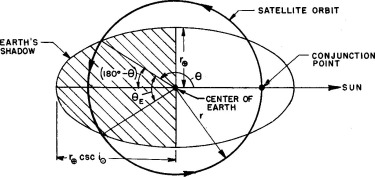
\includegraphics[width=0.6\textwidth]{fig/ssp.jpg}
	\caption[Ilustrasi fase gerhana pada orbit satelit]{Ilustrasi fase gerhana pada orbit satelit~\cite{ismail2015}}
\label{fig:ssp}
\end{center}
\end{figure}

Selanjutnya, posisi sudut satelit terhadap titik \textit{sub-solar} untuk waktu
tertentu dapat dicari dengan mengurangi anomali benar satelit dengan anomali
benar titik \textit{sub-solar}. Gambar \ref{fig:albedofactor} menunjukkan
contoh hasil perhitungan faktor panas akibat albedo.

\begin{figure}[H]
\setlength\belowcaptionskip{-0.7\baselineskip}
\begin{center}
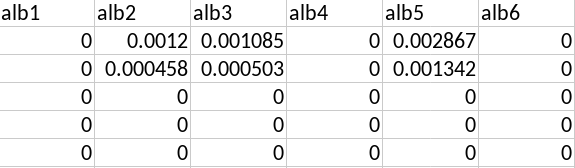
\includegraphics[width=0.6\textwidth]{fig/albedofactor.png}
\caption{Contoh hasil perhitungan faktor panas akibat albedo}
\label{fig:albedofactor}
\end{center}
\end{figure}

Karena \textit{node} 7 pada model satelit LAPAN-A3 mewakili plat tengah satelit
yang diasumsikan terisolasi dari lingkungan luar satelit, laju perubahan suhu
\textit{node} 7 dianggap tidak dipengaruhi faktor panas akibat Matahari,
albedo, maupun Bumi. Diasumsikan juga \textit{node} 7 tidak mengalami disipasi
panas ke lingkungan ruang angkasa sehingga perubahan suhu pada \textit{node} 7
murni terjadi akibat perpindahan panas lewat konduksi dan radiasi dengan
ke-enam \textit{node} lainnya.

\subsection{Penyaringan dataset}

Data gabungan dataset dasar dan hasil perhitungan koefisien faktor termal
satelit kemudian disaring untuk meminimalkan kesalahan dan menghilangkan
\textit{outlier} pembacaan sensor satelit. Kriteria yang digunakan untuk
menyaring dataset adalah sebagai berikut :

\begin{enumerate}
\item Selang waktu antar pengamatan maksimal 120 s 
\item Skor standar suhu \textit{node} satelit memiliki rentang -3 sampai dengan 3
\item Skor standar laju perubahan suhu \textit{node} satelit berkisar dari -3 sampai dengan 3 
\end{enumerate}

Kriteria pertama dipilih berdasarkan persebaran selang waktu pengamatan untuk
data dari kedua periode observasi. Selang waktu pengamatan untuk kedua periode
observasi tidak konstan dan berkisar mulai dari 80 sekon sampai dengan ribuan
sekon. Pada kedua periode observasi, pembacaan sensor kebanyakan memiliki
selang waktu 120 s. Selang waktu lebih besar dari 120 s akibat jeda waktu
pengamatan satelit tidak digunakan karena dapat mengurangi akurasi prediksi
model regresi linear yang akan digunakan. Karena itu, data yang diambil
memiliki selang waktu antar pengamatan maksimal 120 s.

Kriteria kedua dan ketiga dipilih untuk menghilangkan \textit{outlier}
pembacaan sensor satelit. Secara statistik, salah satu cara untuk mengukur
apakah sebuah poin data termasuk dalam kategori \textit{outlier} adalah dengan
menghitung skor standar poin data tersebut. Skor standar $z$ dihitung dengan
membagi selisih antara nilai data $x$ dan rata-rata data $\mu$ dengan standar deviasi
data $\sigma$ seperti pada persamaan berikut \cite{massaron}:

\begin{equation}
\label{eq:zscore}
	z = \frac{x - \mu}{\sigma}
\end{equation}

Skor standar yang terlalu rendah (lebih kecil dari -3) atau tinggi (lebih besar
dari 3) mengindikasikan poin data tersebut dapat dikategorikan \textit{outlier}
\cite{boschetti2015}. Kedua kriteria skor standar mengasumsikan suhu dan laju
perubahan suhu \textit{node-node} satelit terdistribusi secara normal sesuai
dengan asumsi dasar pemodelan regresi linear dalam \textit{machine learning}.
Nilai \textit{outlier} yang ekstrem dapat berpengaruh buruk kepada akurasi
prediksi model sehingga harus dihilangkan dari dataset akhir. Gambar
\ref{fig:cleandataset} menunjukkan contoh dataset yang sudah disaring.

\begin{figure}[H]
\setlength\belowcaptionskip{-0.7\baselineskip}
\begin{center}
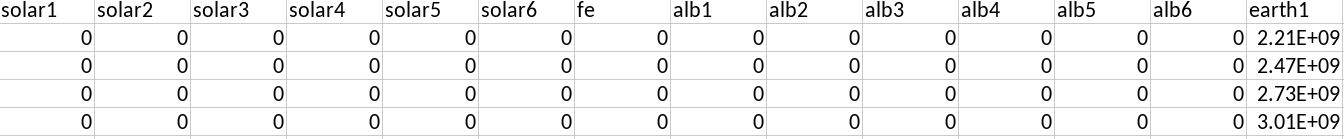
\includegraphics[width=0.8\textwidth]{fig/cleandataset.png}
\caption{Contoh dataset yang sudah disaring}
\label{fig:cleandataset}
\end{center}
\end{figure}


\section{Pelatihan dan Pengujian Model}

Dataset yang sudah disaring kemudian dibagi menjadi set latihan
(\textit{training}) dan ujian (\textit{test}) dengan menggunakan modul
Scikit-learn. Pemodelan pada karya tulis ini menggunakan rasio jumlah data
pelatihan dibanding pengujian sebesar 0.7:0.3 serta pengaturan \textit{seed
number} 0. Tabel \ref{table:dataset} memuat detail jumlah dataset yang
digunakan dalam pemodelan untuk kedua periode observasi.

\begin{table}[!ht]
\begin{center}
\caption{Detail jumlah dataset model \textit{machine learning}}
\label{table:dataset}
\begin{tabular}{|c|cc|}
\hline
\multirow{2}{*}{Tanggal} & \multicolumn{2}{c|}{Dataset}                 \\ \cline{2-3} 
                         & \multicolumn{1}{c|}{Set latihan} & Set ujian \\ \hline
19 Mei 2018              & \multicolumn{1}{c|}{201}         & 87        \\ \hline
20 Mei 2018              & \multicolumn{1}{c|}{180}         & 78        \\ \hline
\end{tabular}
\end{center}
\vspace{-5mm}
\end{table}

Pelatihan dan pengujian model dipisah per tanggal observasi karena pada
Persamaan \ref{eq:lineq} koefisien $c_a$ mengandung nilai sudut bidang orbit
satelit terhadap Matahari $\beta$ yang dianggap konstan selama 1 periode
observasi. Nilai $\beta$ bergantung pada posisi Bumi relatif terhadap Matahari.
Dengan kata lain, nilai $\beta$ berubah seiring dengan pergantian hari
sepanjang tahun akibat revolusi Bumi mengitari Matahari \cite{m2019}.


%Hasil dan Analisis
\chapter{Hasil dan Analisis}

\section{Hasil Pemodelan Termal Satelit LAPAN-A3}

Gambar \ref{fig:node119} sampai dengan \ref{fig:node720} menunjukkan perbandingan suhu \textit{node-node} satelit
hasil prediksi model termal dengan data telemetri LAPAN-A3 aktual untuk periode observasi 19 sampai dengan 20 Mei 2018.

\begin{figure}[H]
\setlength\belowcaptionskip{-0.7\baselineskip}
\begin{center}
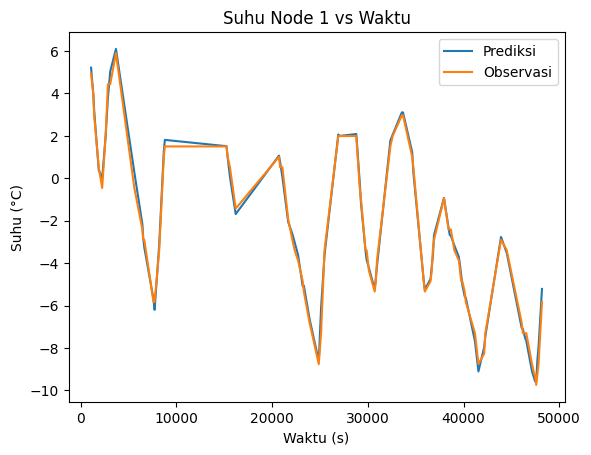
\includegraphics[width=0.6\textwidth]{fig/node1_temp_2018-05-19.png}
	\caption{Grafik suhu \textit{node} 1 vs waktu 19 Mei 2018}
\label{fig:node119}
\end{center}
\end{figure}

\begin{figure}[H]
\setlength\belowcaptionskip{-0.7\baselineskip}
\begin{center}
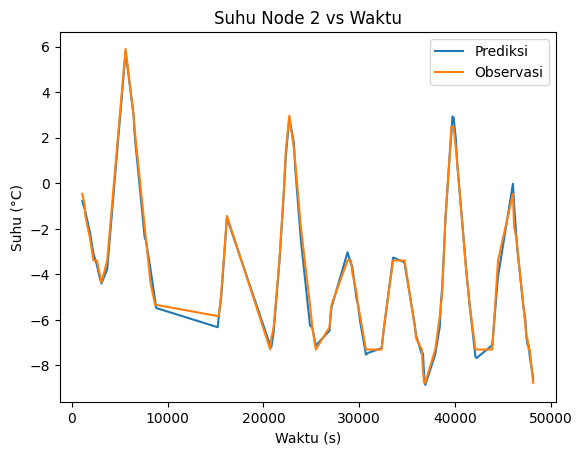
\includegraphics[width=0.6\textwidth]{fig/node2_temp_2018-05-19.png}
	\caption{Grafik suhu \textit{node} 2 vs waktu 19 Mei 2018}
\label{fig:node219}
\end{center}
\end{figure}

\begin{figure}[H]
\setlength\belowcaptionskip{-0.7\baselineskip}
\begin{center}
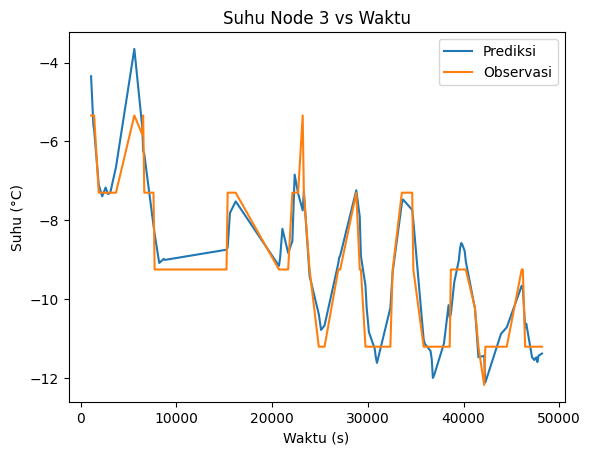
\includegraphics[width=0.6\textwidth]{fig/node3_temp_2018-05-19.png}
	\caption{Grafik suhu \textit{node} 3 vs waktu 19 Mei 2018}
\label{fig:node319}
\end{center}
\end{figure}

\begin{figure}[H]
\setlength\belowcaptionskip{-0.7\baselineskip}
\begin{center}
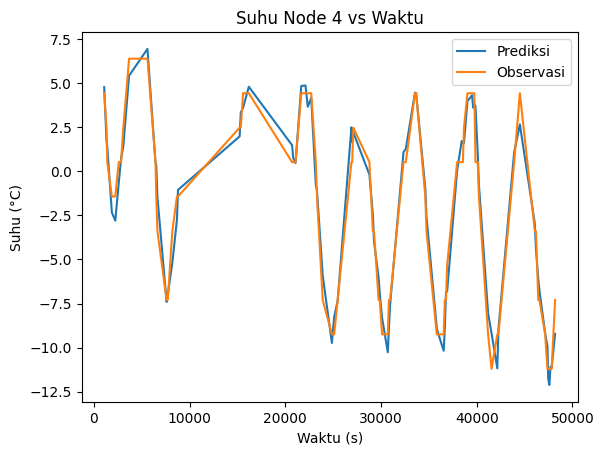
\includegraphics[width=0.6\textwidth]{fig/node4_temp_2018-05-19.png}
	\caption{Grafik suhu \textit{node} 4 vs waktu 19 Mei 2018}
\label{fig:node419}
\end{center}
\end{figure}

\begin{figure}[H]
\setlength\belowcaptionskip{-0.7\baselineskip}
\begin{center}
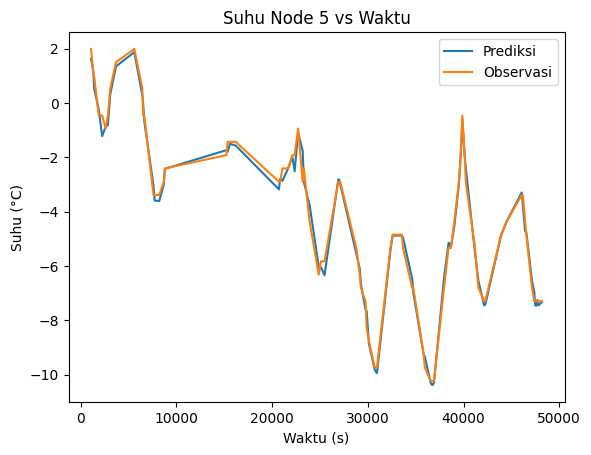
\includegraphics[width=0.6\textwidth]{fig/node5_temp_2018-05-19.png}
	\caption{Grafik suhu \textit{node} 5 vs waktu 19 Mei 2018}
\label{fig:node519}
\end{center}
\end{figure}

\begin{figure}[H]
\setlength\belowcaptionskip{-0.7\baselineskip}
\begin{center}
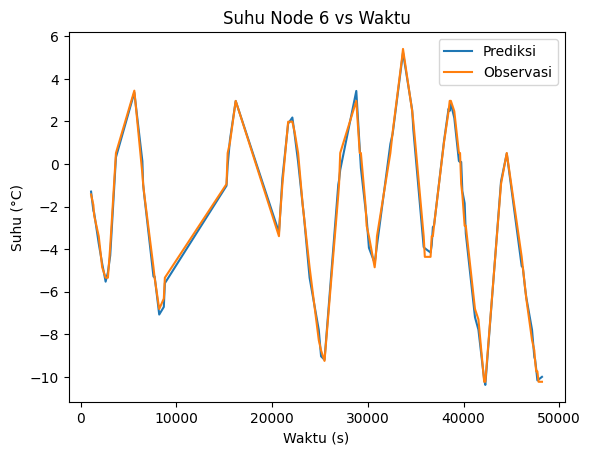
\includegraphics[width=0.6\textwidth]{fig/node6_temp_2018-05-19.png}
	\caption{Grafik suhu \textit{node} 6 vs waktu 19 Mei 2018}
\label{fig:node619}
\end{center}
\end{figure}

\begin{figure}[H]
\setlength\belowcaptionskip{-0.7\baselineskip}
\begin{center}
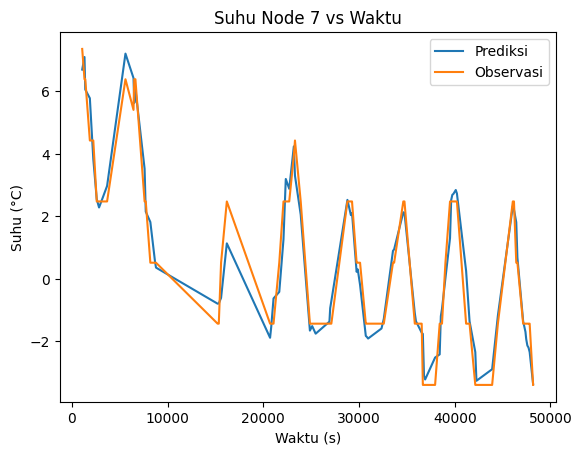
\includegraphics[width=0.6\textwidth]{fig/node7_temp_2018-05-19.png}
\caption{Grafik suhu \textit{node} 7 vs waktu 19 Mei 2018}
\label{fig:node719}
\end{center}
\end{figure}

\begin{figure}[H]
\setlength\belowcaptionskip{-0.7\baselineskip}
\begin{center}
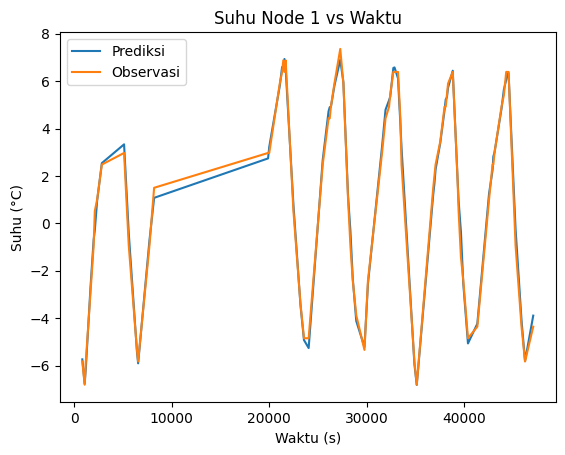
\includegraphics[width=0.6\textwidth]{fig/node1_temp_2018-05-20.png}
\caption{Grafik suhu \textit{node} 1 vs waktu 20 Mei 2018}
\label{fig:node120}
\end{center}
\end{figure}

\begin{figure}[H]
\setlength\belowcaptionskip{-0.7\baselineskip}
\begin{center}
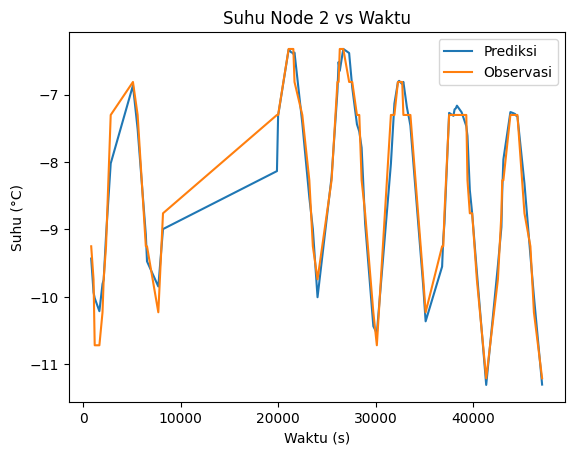
\includegraphics[width=0.6\textwidth]{fig/node2_temp_2018-05-20.png}
\caption{Grafik suhu \textit{node} 2 vs waktu 20 Mei 2018}
\label{fig:node220}
\end{center}
\end{figure}

\begin{figure}[H]
\setlength\belowcaptionskip{-0.7\baselineskip}
\begin{center}
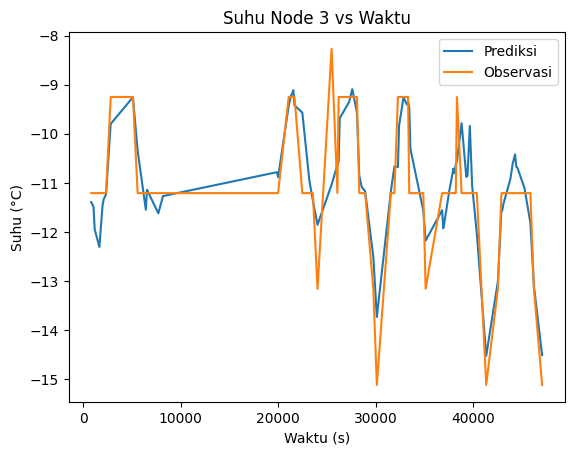
\includegraphics[width=0.6\textwidth]{fig/node3_temp_2018-05-20.png}
\caption{Grafik suhu \textit{node} 3 vs waktu 20 Mei 2018}
\label{fig:node320}
\end{center}
\end{figure}

\begin{figure}[H]
\setlength\belowcaptionskip{-0.7\baselineskip}
\begin{center}
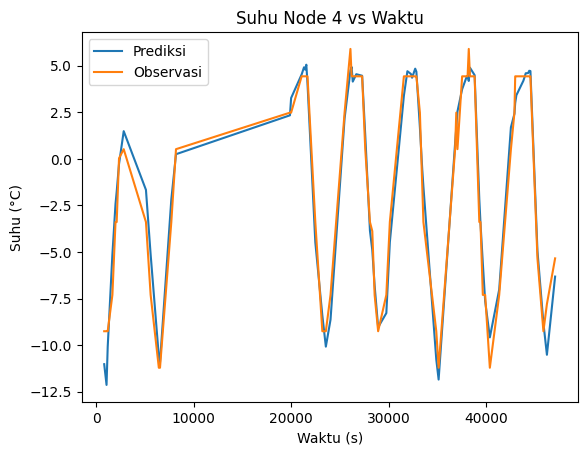
\includegraphics[width=0.6\textwidth]{fig/node4_temp_2018-05-20.png}
\caption{Grafik suhu \textit{node} 4 vs waktu 20 Mei 2018}
\label{fig:node420}
\end{center}
\end{figure}

\begin{figure}[H]
\setlength\belowcaptionskip{-0.7\baselineskip}
\begin{center}
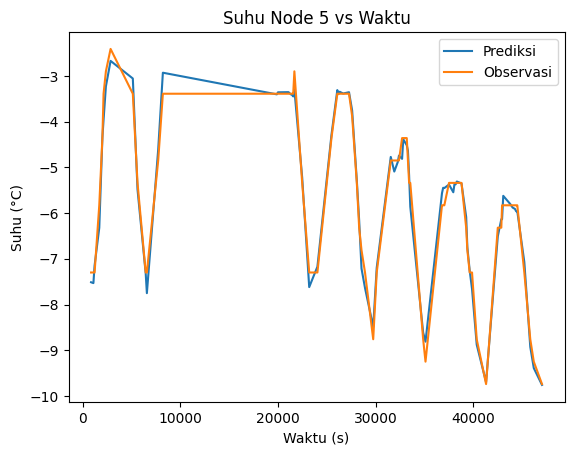
\includegraphics[width=0.6\textwidth]{fig/node5_temp_2018-05-20.png}
\caption{Grafik suhu \textit{node} 5 vs waktu 20 Mei 2018}
\label{fig:node520}
\end{center}
\end{figure}

\begin{figure}[H]
\setlength\belowcaptionskip{-0.7\baselineskip}
\begin{center}
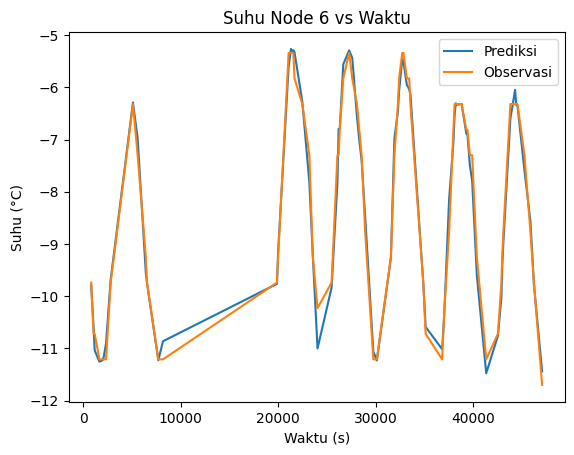
\includegraphics[width=0.6\textwidth]{fig/node6_temp_2018-05-20.png}
\caption{Grafik suhu \textit{node} 6 vs waktu 20 Mei 2018}
\label{fig:node620}
\end{center}
\end{figure}

\begin{figure}[H]
\setlength\belowcaptionskip{-0.7\baselineskip}
\begin{center}
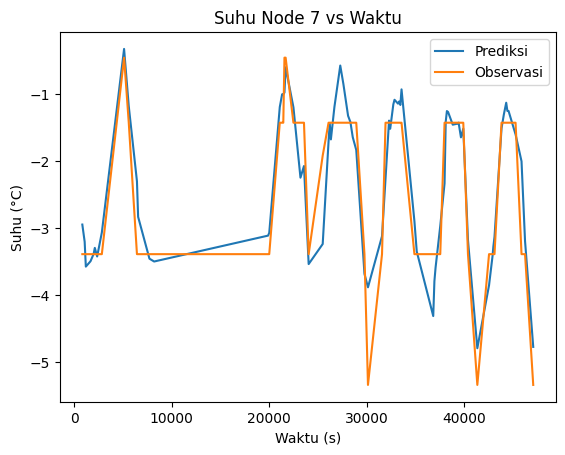
\includegraphics[width=0.6\textwidth]{fig/node7_temp_2018-05-20.png}
\caption{Grafik suhu \textit{node} 7 vs waktu 20 Mei 2018}
\label{fig:node720}
\end{center}
\end{figure}

Dapat dilihat bahwa model termal LAPAN-A3 dapat memprediksi kebanyakan tren
perubahan suhu \textit{node-node} satelit selama periode observasi dengan akurasi yang
cukup dekat dengan suhu observasi. Meskipun prediksi model termal mengalami
\textit{overshoot} dan \textit{undershoot}, model termal secara umum dapat
memprediksi apakah suhu \textit{node-node} satelit akan naik, turun, atau tetap sama
pada setiap selang waktu.

Meski demikian, node 3 dan 7 menghasilkan prediksi suhu
dengan tren yang cukup kontras dengan data suhu observasi. Perbedaan tren
prediksi suhu untuk kedua node terlihat paling jelas pada Gambar \ref{fig:node320}
dan \ref{fig:node720} yang memuat plot suhu \textit{node} 3 dan 7 terhadap waktu untuk
periode observasi 20 Mei 2018. Dari kedua grafik tersebut, dapat dilihat bahwa
model termal memprediksi perubahan suhu \textit{node} meski data telemetri suhu node
konstan seperti yang terjadi pada rentang waktu 10000 sampai dengan 20000
sekon.

Agar dapat dinilai secara kuantitatif, performa model termal dalam memprediksi
tren perubahan suhu \textit{node-node} satelit dapat dilihat dari hasil perhitungan skor koefisien determinasi $R^2$ prediksi suhu \textit{node-node} satelit pada Gambar \ref{fig:r219} dan
\ref{fig:r220}. Model termal LAPAN-A3 dapat menjelaskan mayoritas varians suhu
\textit{node} sehingga menghasilkan skor $R^2$ lebih dari 0.5 untuk semua \textit{node}. Lebih
lanjut, 5 dari 7 \textit{node} pada kedua periode observasi memiliki skor $R^2$ lebih besar dari 0.95. Ini berarti lebih dari 95\%
varians dalam data suhu observasi dapat dijelaskan oleh prediksi model kelima \textit{node} tersebut. Dapat
dilihat juga bahwa \textit{node} 3 memiliki skor $R^2$ paling rendah dari ketujuh \textit{node} pada
kedua periode observasi dan disusul oleh \textit{node} 7.

\begin{figure}[H]
\setlength\belowcaptionskip{-0.7\baselineskip}
\begin{center}
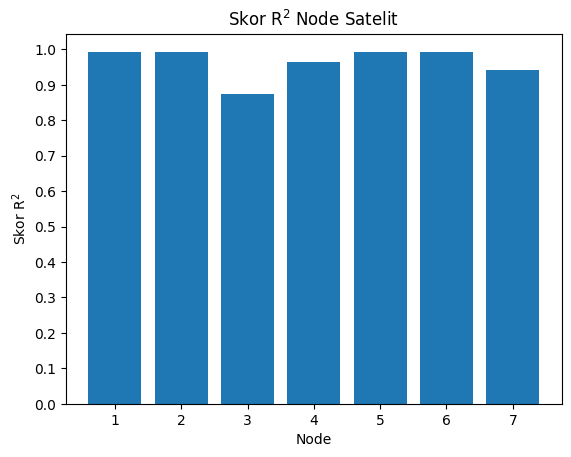
\includegraphics[width=0.6\textwidth]{fig/r2_2018-05-19.png}
\caption{Plot skor $R^2$ model 19 Mei 2018}
\label{fig:r219}
\end{center}
\end{figure}

\begin{figure}[H]
\setlength\belowcaptionskip{-0.7\baselineskip}
\begin{center}
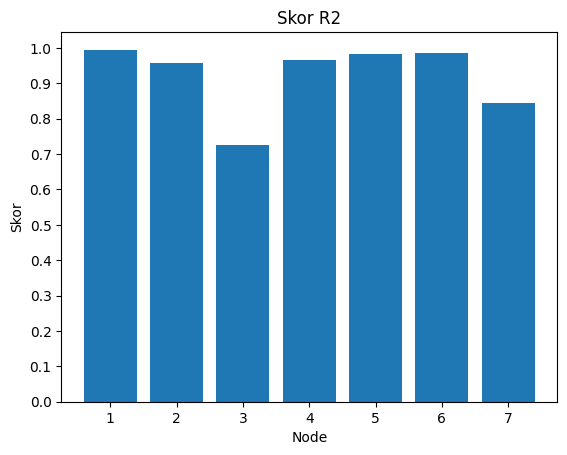
\includegraphics[width=0.6\textwidth]{fig/r2_2018-05-20.png}
\caption{Plot skor $R^2$ model 20 Mei 2018}
\label{fig:r220}
\end{center}
\end{figure}

Selanjutnya, keakuratan model termal dalam memprediksi suhu \textit{node} satelit pada
periode observasi dapat dilihat dari nilai \textit{root mean square error} (RMSE)
model yang mengukur seberapa jauh nilai suhu hasil prediksi model dengan nilai
suhu hasil observasi data telemetri. Gambar \ref{fig:rmse19} dan
\ref{fig:rmse20} memuat plot RMSE model termal. 

\begin{figure}[H]
\setlength\belowcaptionskip{-0.7\baselineskip}
\begin{center}
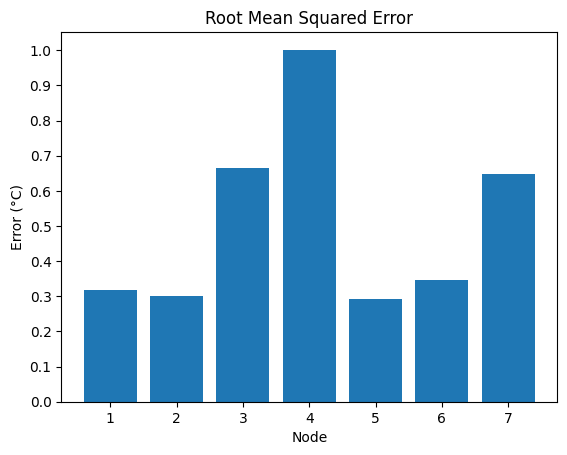
\includegraphics[width=0.6\textwidth]{fig/rmse_2018-05-19.png}
\caption{Plot nilai RMSE model 19 Mei 2018}
\label{fig:rmse19}
\end{center}
\end{figure}

\begin{figure}[H]
\setlength\belowcaptionskip{-0.7\baselineskip}
\begin{center}
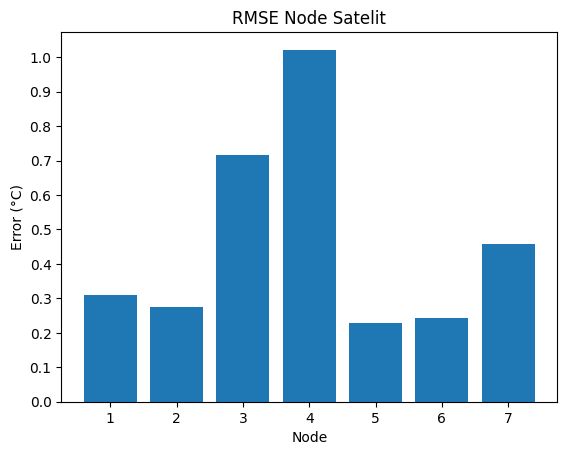
\includegraphics[width=0.6\textwidth]{fig/rmse_2018-05-20.png}
\caption{Plot nilai RMSE model 20 Mei 2018}
\label{fig:rmse20}
\end{center}
\end{figure}

Dapat dilihat bahwa plot RMSE model termal menunjukkan hasil yang agak berbeda
dari plot skor $R^2$ model termal pada Gambar \ref{fig:r219} dan \ref{fig:r220}
sebelumnya. Nilai RMSE paling besar untuk kedua periode observasi sama-sama
diperoleh dari \textit{node} 4 disusul oleh \textit{node} 3 dan kemudian \textit{node} 7. \textit{Node} 4 konsisten
memiliki nilai RMSE lebih besar sedikit dari 1 \degree C untuk kedua periode
observasi. \textit{Node} 3 juga konsisten memiliki nilai RMSE lebih besar dari 0.6
\degree C untuk kedua periode observasi sedangkan \textit{node} 7 sempat menyentuh nilai
di bawah 0.5 \degree C pada periode observasi 20 Mei 2018.

\section{Analisis}

Hasil pemodelan termal satelit LAPAN-A3 dari bagian sebelumnya menunjukkan
bahwa model termal yang dikembangkan sudah dapat memodelkan karakteristik
termal satelit LAPAN-A3 secara umum. Akan tetapi, akurasi model termal satelit
dalam memodelkan karakteristik termal \textit{node} 3, 4, dan 7 dapat dikatakan lebih
rendah dibandingkan dengan 4 \textit{node} lainnya dan masih perlu ditingkatkan. Node 3
dan 7 konsisten memiliki skor $R^2$ lebih rendah dibandingkan \textit{node}-\textit{node} lainnya
sedangkan \textit{node} 4 memiliki nilai RMSE paling besar untuk kedua periode
observasi. Untuk memperjelas letak \textit{node-node} yang akan dianalisis, Gambar \ref{fig:node3}, \ref{fig:node4}, dan \ref{fig:node7} memberikan ilustrasi letak \textit{node} 3, 4, dan 7 pada satelit LAPAN-A3.

\begin{figure}[H]
\setlength\belowcaptionskip{-0.7\baselineskip}
\begin{center}
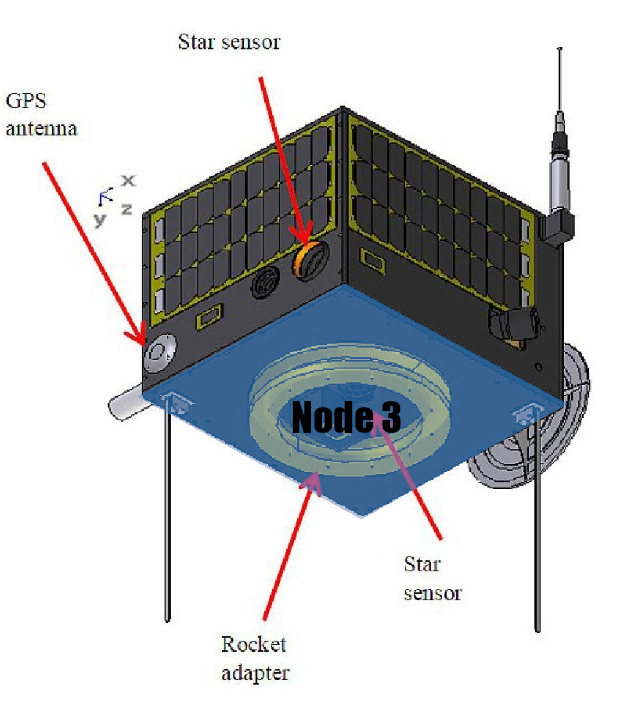
\includegraphics[width=0.6\textwidth]{fig/node3.png}
	\caption{Ilustrasi letak \textit{node} 3 pada satelit LAPAN-A3}
\label{fig:node3}
\end{center}
\end{figure}

\begin{figure}[H]
\setlength\belowcaptionskip{-0.7\baselineskip}
\begin{center}
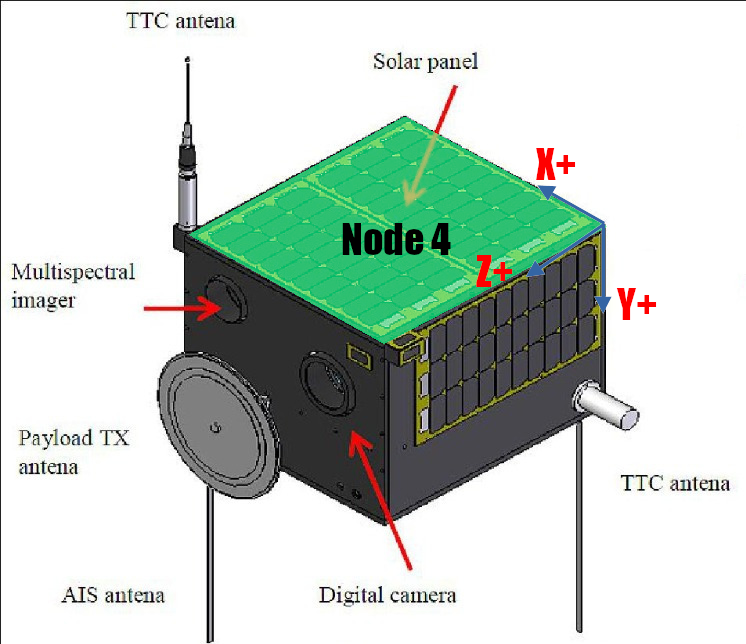
\includegraphics[width=0.6\textwidth]{fig/node4.png}
	\caption{Ilustrasi letak \textit{node} 4 pada satelit LAPAN-A3}
\label{fig:node4}
\end{center}
\end{figure}

\begin{figure}[H]
\setlength\belowcaptionskip{-0.7\baselineskip}
\begin{center}
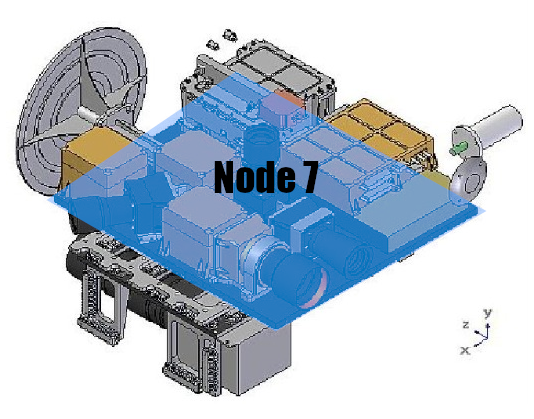
\includegraphics[width=0.6\textwidth]{fig/node7.png}
	\caption{Ilustrasi letak \textit{node} 7 pada satelit LAPAN-A3}
\label{fig:node7}
\end{center}
\end{figure}

Dalam menganalisis hasil pemodelan termal, perlu diingat bahwa metrik performa
model yang dihitung hanya berlaku untuk iterasi dan konfigurasi parameter model
\textit{machine learning} saat ini. Sebagai contoh, perubahan parameter
\textit{seed number} yang digunakan akan mengubah dataset latihan dan ujian
model. Hal ini akan mengubah hasil prediksi model dan tentunya juga akan mengubah
akurasi prediksi model termal. 

Selanjutnya, seperti yang disebutkan pada bab Tinjauan Pustaka, parameter RMSE
bergantung pada skala pemodelan dan dataset yang digunakan. Karena itu,
perbedaan nilai maksimum dan minimum RMSE baru dapat disimpulkan setelah ada
perbandingan dengan model termal di masa depan. Dengan kata lain, belum dapat
disimpulkan apakah nilai RMSE model termal saat ini dapat dikategorikan rendah
atau tinggi.

Terlepas dari ketidakpastian dan ketidakakuratan bawaan dari metode numerik dan
\textit{machine learning} yang digunakan pada karya tulis ini, dapat diduga
bahwa model satelit LAPAN-A3 yang digunakan belum dapat mewakili seluruh
karakteristik termal satelit. Dengan menganalisis sumber ketidakakuratan model
yang potensial, model termal satelit dapat dikembangkan lebih lanjut pada
iterasi berikutnya. Harapannya, iterasi model termal satelit berikutnya dapat
menunjukkan performa yang jauh lebih akurat lagi.

Pertama, satelit LAPAN-A3 didekati dengan model 7 \textit{node} diskrit yang
mewakili 6 sisi satelit serta 1 plat tengah satelit. \textit{Node} digunakan sebagai
satuan titik analisis terkecil sehingga bagian satelit yang diwakili \textit{node}
dianggap memiliki suhu yang sama. Parameter kapasitas termal yang digunakan
pada persamaan-persamaan termal di karya tulis ini pun adalah nilai kapasitas
termal rata-rata \textit{node}. 

\textit{Node} satelit yang terdiri dari material dan komponen yang berbeda dapat
menghasilkan rentang kapasitas termal \textit{node} yang besar juga. Rentang kapasitas
termal yang besar berarti rentang perubahan suhu antar material dalam \textit{node} yang
besar juga. Akibatnya, bacaan sensor suhu bisa saja berbeda jauh dengan suhu
komponen masing-masing sebenarnya.

Dalam konteks LAPAN-A3, seperti yang dapat dilihat pada Gambar \ref{fig:node3} dan \ref{fig:node7}, \textit{node} 3 terletak di sumbu Y+ satelit yang memuat adaptor
roket dan \textit{separation ring} sedangkan \textit{node} 7 terletak di plat tengah
satelit yang menyimpan banyak komponen seperti komputer satelit dan sub-sistem
lainnya. Dengan begitu, karakteristik termal material pada kedua \textit{node} mungkin
tidak dapat terwakili seluruhnya dalam model satelit 7 \textit{node}. Agar karakteristik
termal dapat dimodelkan lebih akurat, jumlah \textit{node} yang digunakan dalam
pemodelan dapat ditambah.

Kemudian, satelit LAPAN-A3 juga diasumsikan berbentuk balok sehingga
perhitungan \textit{view factor} dari \textit{node} ke Bumi disederhanakan
menjadi plat persegi panjang ke Bumi. Pada kenyataannya, satelit memiliki
komponen yang tidak berbentuk persegi panjang seperti antena dan kamera.
Penambahan jumlah \textit{node} untuk memastikan komponen-komponen tersebut
terwakili tentunya juga akan menambah akurasi dari model termal satelit. Selain
itu, tidak tertutup juga penggunaan metode numerik lain seperti metode elemen
hingga untuk menghitung nilai \textit{view factor} secara terpisah agar data
\textit{view factor} yang digunakan untuk melatih model dapat lebih mendekati
nilai \textit{view factor node} satelit yang sebenarnya.

Lalu, dari Persamaan \ref{eq:lineq} dapat dilihat juga bahwa perubahan suhu
suatu \textit{node} dipengaruhi perubahan suhu \textit{node} lain akibat adanya
perpindahan panas lewat konduksi dan radiasi antar \textit{node}. Merujuk
aplikasi lain dari regresi linear pada pemodelan termal satelit, analisis
inferensi dapat dilakukan untuk menentukan variabel-variabel dominan dalam
Persamaan \ref{eq:lineq} yang mungkin menyumbang \textit{error} paling besar.
Jika hasil inferensi menunjukkan bahwa perubahan suhu \textit{node} 4
didominasi oleh pengaruh perubahan suhu \textit{node} 3 dan 7, penjelasan
sebelumnya dapat turut menjawab hasil nilai RMSE \textit{node} 4. Sebaliknya,
hasil analisis tersebut dapat digunakan untuk melihat akurasi suku termal mana
yang perlu ditingkatkan agar perbedaan antara nilai hasil prediksi model dengan
data observasi dapat dikurangi.

Analisis inferensi untuk mengetahui kontribusi tiap variabel dalam Persamaan
\ref{eq:lineq} membutuhkan modifikasi metode \textit{machine learning} yang
digunakan. Dapat dilihat dari persamaan tersebut bahwa variabel suhu
\textit{node} berkorelasi erat dengan variabel suhu \textit{node} pangkat 4.
Jika salah satu variabel diketahui, variabel lainnya dapat dihitung juga.
Fenomena adanya korelasi tinggi antar variabel independen tersebut dinamakan
kolinearitas. 

Meski kolinearitas tidak berdampak banyak pada akurasi prediksi model regresi
linear, hal ini harus diperhitungkan dalam analisis inferensi
\cite{lieberman2014}\cite{mundfrom2018}. Kolinearitas sendiri dapat diatasi
dengan menyeleksi variabel independen sehingga tidak ada kolinearitas pada
variabel yang tersisa atau menggunakan metode \textit{machine learning} lain
yang tidak terpengaruh kolinearitas.

Analisis inferensi persamaan termal tidak dilakukan pada karya tulis ini karena
model termal yang dikembangkan pada karya tulis ini memiliki tujuan utama
berupa prediksi suhu satelit. Meski demikian, topik tersebut dapat menjadi
bahan pengembangan model termal selanjutnya atau topik penelitian lebih lanjut
di masa depan. Dengan begitu, model termal satelit LAPAN-A3 dapat dikembangkan
lebih baik lagi.


%Saran dan Kesimpulan
\chapter{Kesimpulan dan Saran}

\section{Kesimpulan}

Dari penelitian yang dilakukan pada karya tulis ini, didapatkan langkah-langkah
pemodelan termal semi-empiris satelit menggunakan metode \textit{machine learning}.
Algoritma pemodelan termal tersebut diimplementasikan pada model satelit 7 \textit{node}
LAPAN-A3 melalui bahasa pemrograman Python serta dilatih dengan data telemetri
operasi LAPAN-A3 aktual dari 19 sampai dengan 20 Mei 2018. Hasilnya adalah model
termal yang dapat memprediksi suhu satelit LAPAN-A3 selama periode
observasi.

Secara umum, model termal yang dihasilkan dapat memprediksi tren perubahan suhu satelit LAPAN-A3 dengan akurasi yang cukup baik. Hal ini dapat
dilihat dari nilai koefisien determinasi model termal yang lebih besar dari 0.9
untuk 6 dari 7 \textit{node} pada periode observasi 19 Mei 2018 dan 5 dari 7 \textit{node} untuk
20 Mei 2018. Selain itu, 6 dari 7 \textit{node} model termal menghasilkan skor
\textit{root mean square error} kurang dari 1 \degree C untuk kedua periode observasi. 

Meski memiliki beberapa catatan terkait perbaikan performa, model termal yang
dikembangkan di karya tulis ini sudah memenuhi tujuan pembuatan karya tulis
ini. Hasil yang dicapai iterasi model termal akan menjadi \textit{baseline}
untuk performa model termal satelit di masa depan. Dengan demikian, performa
model termal satelit yang dikembangkan dapat terus bertambah semakin akurat.

\section{Saran}

Berikut adalah beberapa saran untuk melanjutkan penelitian karya tulis ini :

\begin{enumerate}
\item Menambah jumlah \textit{node} yang dimodelkan sehingga karakteristik termal satelit dapat termodelkan lebih menyeluruh
\item Mengubah asumsi yang digunakan pada \textit{node} satelit untuk memodelkan perilaku \textit{node} satelit lebih akurat
\item Melakukan analisis lebih lanjut untuk menghitung kontribusi tiap suku dalam persamaan termal satelit
\item Memperpanjang durasi periode observasi sehingga masukan data yang dapat digunakan juga bertambah
\item Menggunakan data dari periode observasi saat satelit melakukan maneuver agar model termal dapat mengakomodasi efek perubahan sikap satelit lebih baik
\end{enumerate}


\newpage
\addcontentsline{toc}{chapter}{Daftar Pustaka}

\bibliography{IEEEabrv,ref}
\end{document}
